\documentclass[lettersize,journal]{IEEEtran}
\usepackage{amsmath,amsfonts}
\usepackage{algorithmic}
\usepackage{algorithm}
\usepackage{array}
\usepackage{geometry}
\usepackage{caption}
\usepackage{longtable}
\usepackage[caption=false,font=normalsize,labelfont=sf,textfont=sf]{subfig}
\usepackage{textcomp}
\usepackage{stfloats}
\usepackage{url}
\usepackage{verbatim}
\usepackage{graphicx}
\usepackage{cite}
\usepackage{tikz}
\usepackage{verbatim}
\usepackage{titlesec}
\usepackage[T1]{fontenc}

\usetikzlibrary{mindmap,trees}
\hyphenation{op-tical net-works semi-conduc-tor IEEE-Xplore}


\newcommand{\subsubsubsection}[1]{%
    \par\medskip
    \noindent\textbf{#1}
    \par\medskip
}

\geometry{margin=1in} % Set margins to ensure the table fits well

\begin{document}

\title{Data-Driven Autonomous Driving Simulation: Survey}
\author{Jayesh Choudhary and Arhan Vora}
\date{17 September 2024}

\maketitle

\begin{abstract}
The Data Driven Autonomous Driving Simulation plays a significant role in development of Autonomous driving as real world testing of autonomous vehicles is very expensive as well as dangerous which presents technical and safety threats along with regulatory challenges.The data driven autonomous driving simulation helps greatly in reducing the expense and safely test and validate the vehicles and thus refine the autonomous vehicles for better and faster growth fulfilling its purpose.

A major problem in advancement of autonomous driving is the upper bound of autonomous driving algorithm's performance, especially in handling extreme and complex driving scenarios due to lack of real world data for such conditions as well as the lack of detailing in the data for such critical cases since the data is generally collected only from cameras instead of using the data from various sensors. The key to overcome this upper bound lies in the data-centric autonomous driving technologies which emphasises the importance of high quality data for diverse conditions in optimizing current algorithms and collecting and utilizing autonomous driving data along with dynamically upgrading it.
The recent advancement in AD simulation, closed loop model training and the increase in data has been a valuable experience. However, the lack of systematic knowledge and deep understanding regarding how to built efficient data-centric autonomous driving technology are still major research gaps.

In this project we understand the state of data-driven autonomous driving simulation and how core technologies like artificial intelligence, machine learning, deep neural networks, sensor data fusion, synthetic data generation for rare but critical cases, integration of real-time data processing capabilities through 5G and edge computing contribute to the growth of autonomous vehicles' performance.

\end{abstract}

\begin{IEEEkeywords}
Data-Driven Autonomous Driving Simulation, Real-World Testing Challenges, Sensor Data Fusion, Synthetic Data Generation, Closed-Loop Model Training, Autonomous Driving Data Collection, Performance Optimization for Self-Driving Cars, Autonomous Driving Algorithms, Simulation-Based Validation, Autonomous Driving Safety
\end{IEEEkeywords}

\section{Introduction}
\IEEEPARstart{A}{utonomous} vehicles (AVs) have become a major focus in research, thanks to its potential of revolutionizing transportation and enhancing road safety \cite{janai2020computer}.One of the most transformative and rapidly growing technologies of the 21st century in the transportation sector is represented by autonomous driving \cite{mirzai2023future}. However, real world on road testing for autonomous vehicles still remains a challenge due to its high costs \cite{NEURIPS2023_1838feeb} , safety issues, scalability, and coverage of rare edge case scenarios. In addition, regulatory hurdles add to the complexity of real-world testing. Moreover, regulatory hurdles add another layer of complexity to real-world experimentation. Data-driven simulation has hence emerged as an indispensible tool to progress the development of autonomous vehicle technology in a safer, more scalable, and cost-effective fashion to develop and validate the system.

Autonomous driving systems are extremely complex by bringing a massive amount of technological surroundings that include sensing, localization, perception, and decision making \cite{liu2017computer}. In addition, the application relies absolutely on the seamless interaction, which needs to happen between cloud platforms, huge data storages, and HD maps \cite{liu2017computer}.

Though promising, autodriving technology faces a major performance hurdle given the current limitations of algorithms and the complexity of real-world driving conditions  \cite{li2023datacentric}. Data-driven simulation relies on the vast amount of real-world driving data from cameras, sensor inputs, artificial intelligence, machine learning models to create highly realistic virtual environments. These simulations allow developers to test autonomous driving in a vast variety of scenarios- like heavy traffic, rare conditions like natural disasters, extreme weather conditions, interaction with erratic drivers- which are difficult to test in real world. By improving algorithms in a controlled virtual environment, developers can enhance the performance of autonomous vehicle systems while reducing the danger and expense.

One of the major obstacles in the growth of AVs is the limitation of real world data, especially for rare and extreme driving situations.  90\% of the autonomous driving data received is for normal driving scenarios \cite{ref1}. Autonomous vehicles lack sufficient data to train their models for critical cases that do not occur often. These unusual, however critical scenarios help in training AV models to deal with the unexpected situation so that self-driving systems are secure and more reliable. In the event of an encounter with too few exposures towards these edge cases, AVs may fail to properly react at critical times.
This issue is further complicated by the fact that most of training data is from lesser variety of sensors, particularly cameras leaving out essential information from other sensors \cite{ref1}. This lack of diverse sensor data leaves gaps in spatial understanding and reduces the robustness of AV systems when complex driving conditions arise in front of them. Overcoming these limitations requires more data from extreme driving scenarios and the integration of multi-sensor data to form a basis for more resilient and adaptable autonomous systems.

Later progresses in high-fidelity test systems presently make it conceivable to prepare independent driving operators in closed circle, possibly circumventing inside and out the unmanageable issue of how to control the conveyance move that arises between training and deployment, and enabling scaling of training both safely and very cheaply. There is relatively little known about how to build benchmarking aids to train in closed-loop settings. \cite{zhang2022rethinking}.

Our research focuses on the use of next generation technologies to improve and develop data-driven autonomous driving simulators, with a focus on advanced machine learning techniques in sensor fusion and on-generation synthetic data for some of the very rarest or most hazardous scenarios. Synthetic data, as such, is useful to create realistic simulations of challenging conditions that would be hard or impossible to replicate in real world experiments. Such simulation enables training in a well-controlled, safe environment and therefore increases the robustness and reliability of autonomous systems.

Emerging trends further enrich this landscape of simulations. As 5G and edge computing start to come into the picture for real-time processing, simulation fidelity, as well as the responsiveness of simulations, has been taken to new heights - enable a machine system to process and answer information more quickly and accurately. Human-AI collaboration is moreover of tall significance, since human-in-the-loop frameworks reveal imperative disclosures on intelligent between independent and human drivers to move forward more secure and more agreeable driving situations.

This development, however comes with huge challenges: knowledge and models developed in simulation must be successfully transferred to real applications. This will call for techniques like domain adaptation and generalization to ensure efficient bridging between virtual and real-world performances. There is also a need to bring to the fore the regulatory standards of simulation frameworks, which change over time, along with critical ethical questions such as fairness, bias reduction, and accountability within AI decision-making.


\begin{figure}[h]
    \centering
    \resizebox{\linewidth}{!}{ % Resizes the image to fit within the text width
    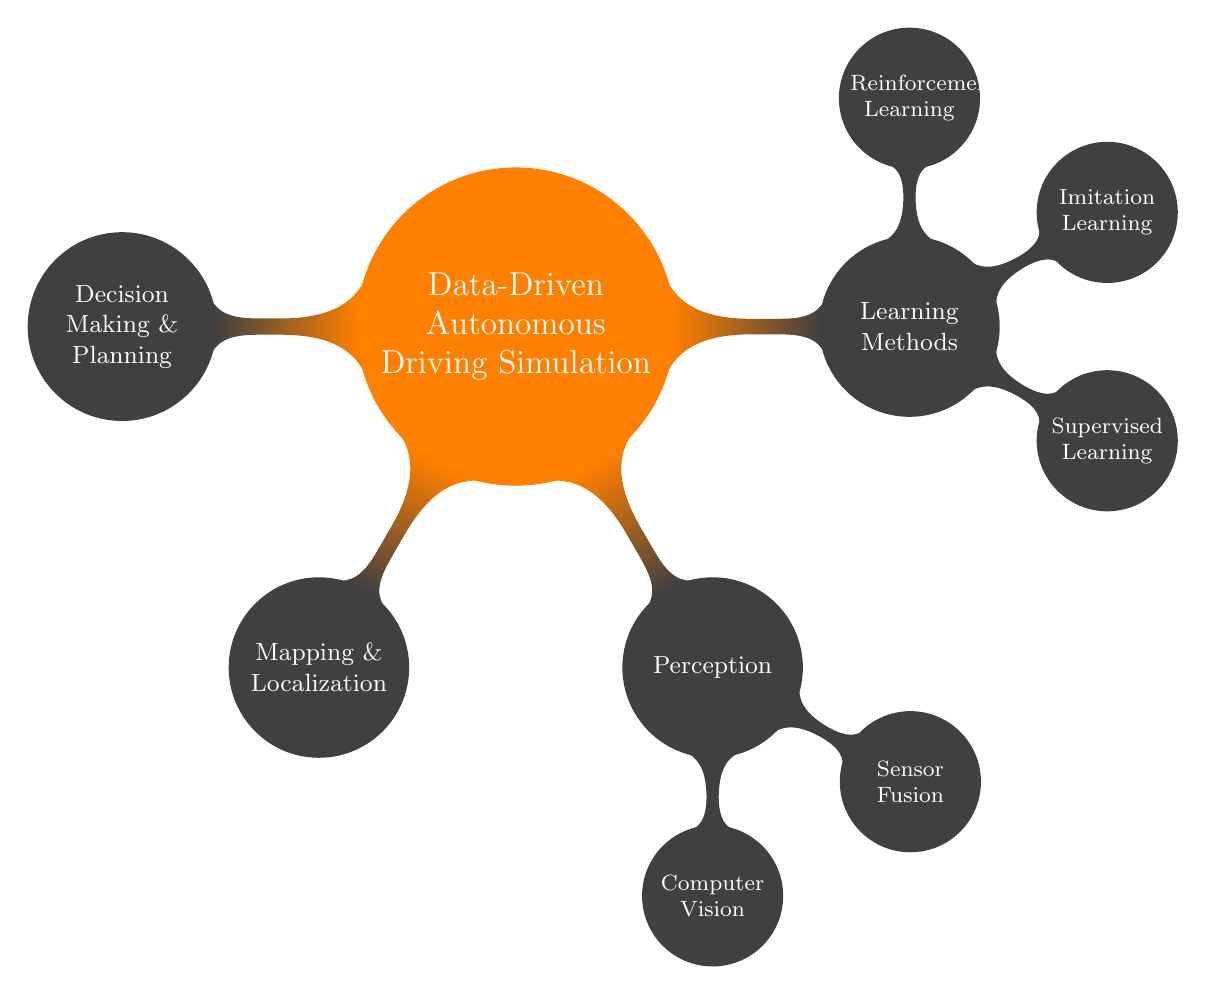
\begin{tikzpicture}
      \path[mindmap,concept color=orange,text=white]
        node[concept] {Data-Driven Autonomous\\Driving Simulation}
        [clockwise from=0]
        child[concept color=gray!50!black] {
          node[concept] {Learning Methods}
          [clockwise from=90]
          child { node[concept] {Reinforcement Learning} }
          child { node[concept] {Imitation Learning} }
          child { node[concept] {Supervised Learning} }
        }
        child[concept color=gray!50!black] {
          node[concept] {Perception}
          [clockwise from=-30]
          child { node[concept] {Sensor Fusion} }
          child { node[concept] {Computer Vision} }
        }
        child[concept color=gray!50!black] { node[concept] {Mapping \& Localization} }
        child[concept color=gray!50!black] { node[concept] {Decision Making \& Planning} };
    \end{tikzpicture}
    }
    \caption{Mind map of data-driven autonomous driving simulation technologies.}
    \label{fig:mindmap}
\end{figure}

\section{Literature Search and Selection}
\subsection{Search Strategy}
\subsubsection{Sources and Databases}
We have used sources, including Google Scholar, IEEE Xplore, ScienceDirect, CiteSeerX, ACM Digital Library, and SpringerLink. These have many quality research papers presented in the top conference across the globe and, hence, have proven to be excellent resources for this project.

\subsubsection{GitHub}
Papers have also been cross-referenced from GitHub repositories such as Awesome Data Centric Autonomous Driving by LincanLi98, End-to-End Autonomous Driving from OpenDriveLab, and related papers from the page on SafeAV's GitHub page.

\subsubsection{Search Terms}
The keywords used to filter the search results include:
\begin{itemize}
    \item Autonomous Driving
    \item Autonomous Driving Simulations
    \item Data-Driven Driving Simulations
    \item ML-based Driving
    \item Intelligent Driving Systems
    \item Algorithms for Autonomous Driving
\end{itemize}

\subsubsection{Time Frame}
Our focus was on papers published in the last decade, specifically from 2014 to 2024.

\subsection{Inclusion Criteria}
\subsubsection{Relevance}
We are in this study to bring on board research aimed at addressing the use of different machine learning models and algorithms towards achieving autonomous driving systems. Again, the paper should share information on improving efficiency through data training on the models while the testing phase rotates around the simulations used to analyze their performance.

\subsubsection{Quality}
 The articles should have huge impact and applications on real world research-projects. Refer from sources which have gone through rigorous reviewing and have been validated by experts in the field.

\subsubsection{Publication Type}
Only quality research papers and published articles that have been accepted and passed through peer review by experts in the same field are used. Also, conference papers, conclusions from reliable and trustworthy sources, and technical reports that have been verified also come within this category.

\subsection{Exclusion Criteria}
\subsubsection{Irrelevance}
Studies which do not focus on Data Driven Autonomous Driving Simulation, it's application or reviews. The study should be aligned with the central theme of our review. Articles without a clear connection to our topic of research and those without any clear conclusion or insights should be excluded.

\subsubsection{Quality}
Exclude studies which are controversial, have proven flaws, have low credibility, showcase insufficient data. Papers which have an unclear focus, questionable assumptions, bad design, unprofessional content should be excluded.

\subsubsection{Publication Type}
Articles published by sources that are not trustworthy, non-technical publishers, articles that have not been reviewed, opinions, and incomplete research results were not be included.

\subsection{Screening}
We started screening for study selection by searching the mentioned keywords across multiple research databases.
Then we proceeded to screen them on basis of the relevance to the topic and credibility scores. We filtered out
the papers which were irrelevant to our topic and those which had low credibility. Next we filtered out those which
did not prove to be up to the quality standards set by us as described above. We then started to go through these
research papers and started extracting the information from these selected sources and integrated them into our own
survey report providing appropriate references and citations.
This approach guaranteed that we not only covered a wide range of diverse studies on the topic but also covered the
topic in depth allowing us to present an in-depth comprehensive analysis report for the wide range of topics included.
As a result we not only covered the breadth of the subject but also reached an appropriate depth in the subject.







% For 50% Submission
\section{Review of Literature}
\subsection{Thematic Organization}
This is a study into data-driven simulation for autonomous driving. Its scope covers the field of development and optimization through autonomous vehicles. This research focuses on some core technologies: artificial intelligence, deep neural networks, sensor data fusion, and generation of synthetic data through techniques in machine learning-all relating to autonomously driven vehicles and crucial to the improvement of performance under variously complex situations. It also takes into consideration the 5G and edge computing, which makes it possible to process and integrate data in real-time, by taking into account the challenges and what has been achieved so far in the area.

The key objective of this study is to synthesize and understand the present state of data-driven autonomous driving simulation and its contribution in overcoming upper performance limits of autonomous driving algorithms. In more detail, the study investigates how the use of high-quality data in combination with real-time processing capabilities and synthetic generation of rare and critical scenarios can enhance the performance of autonomous vehicles. The study also aims to identify the gaps in systematic knowledge called upon in the development of efficient data-centric autonomous driving technologies and propose solutions to fill those gaps.
\\

\subsubsection{Key Themes and Topics Appearing Repeatedly}

\subsubsubsection{1. High-Fidelity Traffic and Behavior Modeling}
The need to capture realistic and high-fidelity traffic models for effective simulation is a recurrent theme within several of the papers. This is something important to consider because traditional simulations often do not have enough scope to capture the richness of multi-agent environments or vehicle-to-vehicle interactions.
Approaches that use methods like LSTM encoding-decoding with attention mechanisms \cite{ref2} or exploiting existing real-world datasets in public domains \cite{ref4} resemble the fine-grained behaviors of vehicles under multivariate settings.
These models are crucial toward making realistic and trustworthy simulations that underlie the complexities and dynamics of road scenarios.
\\
\subsubsubsection{2. Data-Driven Simulation Engines}
Here, the most repeated idea is the use of data-driven simulation engines to enhance algorithmic development for autonomous driving. It simulates real-world conditions through the use of a large dataset within these engines.
For instance, the Waymax simulator \cite{ref4}, has been designed to scale well with large datasets. It can handle hundreds of thousands of events, an example of these is the Waymo Open Motion Dataset. Additionally, it is designed for large-scale, multi-agent simulation of scenes. Its support for running on accelerators such as TPUs and GPUs further supports real-time scalable workflows for machine learning.
\\
\subsubsubsection{3. Reinforcement Learning and Policy Learning in Simulation}
There are several papers which have used the use of reinforcement learning (RL) and imitation learning to train the policies of autonomous driving within simulated environments. These policies enable the agents to generalize the real-world unseen scenarios, such as new roads or near-crash situations.
In \cite{ref3}, through data-driven simulation systems, they were able to demonstrate how they can generate virtual trajectories that help the autonomous vehicles navigate complex and unseen environments and test their policies in simulation tests and real-world tests.
Such a trend toward using RL within simulation while learning policy underlines the increased importance of robust and scalable simulation systems capable of managing complex interaction-rich environments.
\\
\subsubsubsection{4. Challenges in Realism and Sim-to-Real Transfer}
While simulation has its significant advantages for safe, cost-effective testing, challenges arise in realism -- specifically regarding perception realism (proper sensing of the environment) and behavior realism (adequate mimicry of human-like driving behaviors).
Papers mention the limitations in the current simulators, like not simulating complex multi-agent interactions and failing to capture the challenging edge cases due to a lack of real-world data for such scenarios (for example, \cite{ref5}).
To bridge that gap, simulators are increasingly turning to high-fidelity data synthesis and generative models to step away from model-based simulations. The data-driven approaches promise higher data-efficiency and better generalization towards the real world of driving.
\\
\subsubsubsection{5. Simulators for Validation and Benchmarking}
Some of the simulators, such as Waymax in \cite{ref4} and the rest of those outlined in section 4, also highlight their function besides training purposes-for validation and benchmarking of autonomous driving algorithms.
They allow for cross-validation of various algorithms, RL and imitation learning models. Ablation studies and benchmarking experiments are provided by these simulators.
\\
\subsubsubsection{6. Complexity and Interplay between Agents}
There are also critical paper points indicating that rare yet critical scenarios—near collision, for example, or complex multi-agent interactions—are still big challenges. Algorithms often lack data in such situations because of the complexity of maneuvering autonomous vehicles, making simulators more crucial for generating synthetic data and inpainting challenging scenarios.
This focus on multi-agent interactions is very important for enhancing autonomous driving in changing traffic environments. Data-driven techniques are primarily required to achieve realistic interactions between vehicles and to ensure that policies transfer well from simulation to real-world environments \cite{ref5}.
\\
\\



\subsubsection{Synthesis for Literature Review}

\subsubsubsection{Introduction and Objective}
The review is intended for the purpose of understanding the role that data-driven autonomous driving simulations play in optimizing autonomous vehicle performance in the context of high-fidelity traffic modeling, scalable policy learning techniques, and overcoming real-world data transfer challenges and realism.
\\
\\
\subsubsubsection{Theme 1: High-Fidelity Simulation and Traffic Modeling}
\textbf{Introduction:}
The review is intended for the purpose of understanding the role that data-driven autonomous driving simulations play in optimizing autonomous vehicle performance in the context of high-fidelity traffic modeling, scalable policy learning techniques, and overcoming real-world data transfer challenges and realism.

\textbf{Analysis:}  \\
\textbf{Agreement:}
Researchers by and large tend to agree that the traffic modeling is very pivotal to enhance the fidelity of simulation environments utilized in testing autonomous driving systems. This happens through mainly accurate modeling of vehicle-vehicle interactions, especially in complicated scenarios involving multiple interacting vehicles. There is agreement that spatiotemporal dynamics of traffic should be captured to make high-fidelity models.

\textbf{Argument:}
Most of the papers emphasized the importance of accurately predicting the traffic model. However, there are differences about approaches that entail specific techniques-mostly on LSTM with attention mechanisms-like in \cite{ref2} while others used traditional methods for the traffic data modeling, such as \cite{ref2},\cite{ref9} can be considered. Besides, the debate over whether system-level traffic modeling \cite{ref2} outperforms individual vehicle-centric models carries forward a research gap.

\textbf{Evidence:}
\cite{ref2}'s methodology, which uses LSTM and multi-head attention to simulate traffic interactions, is strong in terms of empirical evidence from experimental results. Though \cite{ref2} introduces novel system-based modelling, it also shows robustness in handling complexity, though relatively weaker in generality to different environments for various types of traffics. There are some studies that rely on more traditional approaches and can be less convincing when the extremes of traffic or subtle vehicle interaction behavior are considered.

\textbf{Synthesis:}
Overall, across the papers, there appears to be a theme: a growing awareness of the need for dynamic system-level traffic models incorporating realistic vehicle interactions. There is a trend toward machine learning-based methods, such as LSTM, in showing how the field is becoming increasingly complex in order to accommodate multi-agent interactions. Collectively, the papers seem to point out that though fidelity in the traffic models is improving, there does exist a challenge of generalization to unseen scenarios.
\\
\\

\subsubsubsection{Theme 2: Data-Driven Simulation Engines and Reinforcement Learning}
\textbf{Introduction:}
The data-driven engines have now been utilized in exploiting large sets for learning driving policies. These simulations would then let an autonomous vehicle learn and generalize from new conditions on the roads using reinforcement learning without requiring massive human supervision.

\textbf{Analysis:}  \\
\textbf{Agreement:}
Most researchers believe that simulation engines fueled with reinforcement learning (RL) driven by data play a crucial role in training autonomous vehicles efficiently. These engines capitalize on large amounts of data in building up the driving behaviors of the system and optimize the learning efficiency to represent alternative proposals that come with savings of exorbitant costs as opposed to the real-world testing. RL is highly focused upon its capability towards providing optimization for the drive policies by virtue of iterative simulations.

\textbf{Argument:}
The disagreement lies in the fact that the usage of data-driven engines is impracticable or rather obsolete when it is based on rare-edge case scenarios. These simulators are said to perform quite well for few events of driving as reported by some papers, such as \cite{ref5}, whereas others say that small datasets will not be able to provide edge cases appropriately as concluded by others like \cite{ref4}. Another debate will be the scalability of the such RL-based engines. The papers like \cite{ref4} rely very much on scalability to large data that Waymax presents whereas it has been brought into debate as computationally infeasible to carry out this simulation on large scales.


\textbf{Evidence:}
Papers like \cite{ref5} and \cite{ref4} have enough strong experimental evidence to show the scalability of data-driven simulation engines. To that, they use publicly released driving datasets and hardware accelerators, TPU/GPUs. Smaller datasets that do not contain diverse scenarios that \cite{ref5} speaks about are perhaps some bottlenecks in working with less data that perhaps models are incomplete and biased for engines relying on less data.

\textbf{Synthesis:}
Overall, the general impression is that data-centric engines, and particularly in the scenario with RL, are revolutionizing the simulation of autonomous vehicles. Overall, the combination of papers indicates a scaling trend within both the size of data and the complexity of scenarios, where RL constitutes an extremely efficient means of learning and fine-tuning driving policies. On the other hand, however, limitations placed on the dataset can be the obstacle in the handling of rare and complex driving events.
\\
\\
\subsubsubsection{Theme 3: Challenges and Limitations in Sim-to-Real Transfer}
\textbf{Introduction:}
Even though the technology available today is much advanced, simulators still find it very challenging to approach real life and edge cases, especially when it comes to robust autonomous driving. The need for high-fidelity data generation coupled with efficient sim-to-real transfer mechanisms can break these barriers.

\textbf{Analysis:} \\
\textbf{Agreement:}
All papers agree that sim-to-real transfer is challenging for autonomous driving. It is hard to apply directly the model trained in the simulation data onto real-world conditions. Most authors agree that domain randomization or data augmentation techniques must be applied to bridge this gap.

\textbf{Argument:}
The principle debate is with regard to how to best bridge the domain gap. While \cite{ref5} strongly claims that inpainting and synthetic data generation can be sufficient solutions to the challenge, especially if one does not need to resort to domain randomization, other approaches emphasize that for higher realism, more robust solutions, such as multi-sensor data fusion, will be needed-thus said the author of \cite{ref2}. Very controversial is again the point of whether real-time simulation updates are necessary (e.g., \cite{ref4}, \cite{ref5}) for successful sim-to-real transfer or whether batched processing of the simulation outcomes is enough.


\textbf{Evidence:}
Strength of Evidence \cite{ref5} had reasonably strong empirical evidence as it successfully demonstrated sim-to-real transfer without domain randomization, and synthetic data could be used in reinforcement learning environments. However, its results are context-dependent and are likely to be less generalizable for the highly dynamic environment found in reality. Papers on multi-sensor fusion present a more robust solution but offer less experimentation validation.

\textbf{Synthesis:}
Most of the papers have an increasing trend towards an improvement of sim-to-real transfer by utilizing advanced simulation techniques including inpainting, sensor fusion, and data augmentation. On one hand, the field is trending toward even more realistic simulations that are close to sensor-accurate, but there is still a gap within that makes it seem impossible to achieve seamless transfer to real-world applications, especially those found in edge cases and complex environments.
\\
\\
\subsubsubsection{Theme 4: Multi-Agent Interaction and Complex Scenario Handling}
\textbf{Introduction:}
Managing interactions of many agents and extreme scenarios remains a critical issue. Data-driven approaches, which produce synthetic data to handle such sparse cases, become even more central towards improving policy robustness and warranting safe real-world deployment of autonomous systems.
\textbf{Analysis:}  \\
\textbf{Agreement:}
Experts agree that there is a need to simulate complex scenarios and manage multi-agent interactions for self-driving car research. Surprisingly enough, potential interaction cases with other cars or pedestrians as well as unforeseen occurrences are usually ranked as the most challenging testing case for such automobiles.

\textbf{Argument:}
There is near unanimity in the fact that one should study multi-agent interactions, but there is disagreement about how to do so better. For example, papers such as \cite{ref4} would argue that data-efficient simulators are suitable for such tasks, while others would argue that the simulators used until now, such as in \cite{ref9}, do not contain the appropriate levels of complexity to represent real-world interactions. Another type of dispute arises when trying to choose between pre-defined scenario-based simulations and dynamic simulation environments which change their complexity in real-time.


\textbf{Evidence:}
Only the more comprehensive papers with big data, like \cite{ref4} and its use of Waymax data, truly are strong; others, especially those with data of smaller size may lack in complexity for multi-agent interactions. In cases where synthetic data is generated for edge cases, it really becomes a solid approach, at least as seen in \cite{ref5}, but refinement may be a necessity to get closer to realistic behaviors in a real-world context.

\textbf{Synthesis:}
 Papers were trending toward more complex datasets with edge cases and better dynamic scene generation to enhance multi-agent interaction simulations. Collectively, these papers suggested that high-fidelity interaction modeling was still developing with respect to better edge case representation; however, scalability and data diversity remain the biggest challenges toward simulating real-world complexity in fully developed methods.
\\
\\
\subsubsubsection{Theme 5: Sim-to-Real Transfer and Domain Adaptation}
\textbf{Introduction:}
Much of the papers emphasize the requirement for sim-to-real transfer - that is, take a policy or model trained in simulation and deploy it successfully in the real world. This process tends to be complicated by the nature of the domain gap that exists between synthetic data commonly used in simulation and real-world environments. Papers on the theme of reinforcement learning and synthetic data describe methods for crossing this gap, including inpainting, domain randomization, and real-time semantic segmentation (e.g., \cite{ref10}). In particular, successful transfer without domain randomization \cite{ref5} is a key highlight, which recommends that simulation engines are moving closer to bridging the gap between virtual and real-world applications.

\textbf{Analysis:}  \\
\textbf{Agreement:}
It is almost a unanimous consensus among the researchers that transferring sim-to-real is important for the successful deployment of simulation-trained autonomous systems in the real world. Attention turns to closing the domain gap with domain randomization, inpainting, and other techniques that generate synthetic data.

\textbf{Argument:}
Some authors-\cite{ref5}-contend that synthetic data is inherently sufficient to cross the sim-to-real gap, while others believe it must be combined with real sensor data in order to build greater realism of simulation. This debate also extends to whether current simulators are capable of supporting such transfer at scale, with some of the papers insisting they cannot attain the necessary complexity.


\textbf{Evidence:}
The main strength of \cite{ref5} is the fact that it has succeeded in demonstrating sim-to-real transfer without the use of domain randomization, making its evidence highly attractive to the scenarios the use of synthetic data would depict. Its application, however, is unlikely to be upgraded to more complex driving situations because of the fact that apparently more significant contributions from other studies as well as to real-time updates for simulation would seem to afford a firmer ground for long-term solutions in this regard.


\textbf{Synthesis:}
The overall trend is towards sim-to-real gaps that are narrower in nature through more complex simulation engines and synthesis data techniques. That being said, although domain randomization is still useful, some of the newer data-efficient simulation strategies such as inpainting and real-time perception modeling will eventually move this functionality in.
\\
\\
\subsubsubsection{Theme 6: Perception Realism and Sensor Data Fusion}
\textbf{Introduction:}
Abstracts in several places discuss the realism of perception systems in simulators, focusing on how they replicate sensor data from cameras, LIDAR, or radar.
Such simulation systems as \cite{ref11}, pursuing the imitation of human-like perception, can be of special help for the assessment of driving behaviors under realistic traffic environments. These simulators emphasize the generation of data that reflect real-world sensor inputs; hence, this system is important to train policies performing well in reality.
In addition to the above approaches, incorporating sensor data to reinforcement learning \cite{ref10} or improving visual sensor fidelity \cite{ref11} enhance more realism and reliability in autonomous driving simulations.

\textbf{Analysis:}  \\
\textbf{Agreement:}
It is agreed that fidelity of sensor data and realism of perception are important in simulation for autonomous driving. The simulators have to mimic sensor data in the real world coming from cameras, LIDAR, or radar inputs to possibly train and validate the autonomy systems accurately.

\textbf{Argument:}
Are perception systems currently good enough for high-fidelity simulation? According to \cite{ref11}, simulators are currently deficient in perception realism on traffic scene data. \cite{ref2} proposes sensor fusion as a technique for heightening the accuracy of these simulations. \cite{ref10} has synthetic perception data with more reliance.


\textbf{Evidence:}
Papers advocating for sensor fusion, as a for instance, \cite{ref2}, go with strong theoretical justification, but lack proper experimental evidence in highly complex real-world settings. The synthetic perception approach, for instance, \cite{ref10}, are known to have some success in narrow tests, but are in need of further validation in highly diverse environments.

\textbf{Synthesis:}
Improvement in perception realism follows through with assimilation of multi-sensor data and richer scenes simulations of the real world. Some simulators aim to generate synthetic data, while increasing recognition for sensor fusion can provide a better comprehensive solution to the problem of high fidelity simulation of perception systems.
\\
\\
\subsection{Critical Analysis}
\textbf{Methodologies:}

\textbf{High-fidelity Simulation and Traffic Modeling:}
\begin{itemize}
    \item \textbf{Strengths:} \cite{ref2} implements the machine-learning model, like LSTM with the multi-head attention mechanism. This methodology of using such models on vehicles will capture the complex spatiotemporal interaction. The stage at which initial data is available helps enhance the simulated output by training of models from traffic data. The system-based modeling approach concerning traffic was proposed in \cite{ref2} and reflects an advanced method by considering overall traffic instead of any individual vehicle.
    \item \textbf{Weaknesses:} These models often rely on small datasets and, although capturing short-term dependencies well, might not generalize over divers or rare edge-case scenarios. Also, data screening based on traffic metrics could imply training biases in models since there is too much reliance on predefined complexities in traffic and not enough on looking for outliers.
\end{itemize}

\vspace{1em} % Adjust the amount of space as needed

\textbf{Data-Driven Simulation Engines and Reinforcement Learning:}
\begin{itemize}
    \item \textbf{Strengths:} Data-driven approaches based on reinforcement learning (RL) \cite{ref3}, \cite{ref5} provide scalable and robust frameworks for training policies for autonomous vehicles. RL's adaptability to novel settings and ability to learn through trial and error are a good fit with driving environments. The synthetic data generated within simulation engines is richly exploitable in order to carry out ample testing without needing a real-world data acquisition cost, \cite{ref10}. The novel inpainting and scene rendering-based approach for sparse reward training has the potential to be scalable in simulations, \cite{ref5}.
    \item \textbf{Weakness:} Many RL-based simulation engines suffer from significant computational bottlenecks that necessitate large-scale hardware accelerators, like TPUs/GPUs \cite{ref4}. Theoretically, the frameworks are robust; however, they will be impractical for small research groups or industries with no access to abundant resources. Further, use of sparse rewards and simulated environments results in overfitting wherein good performances in simulations result in poor realism.
\end{itemize}

\vspace{1em}

\textbf{Simulations-to-Real Transfer:}
\begin{itemize}
    \item \textbf{Strengths:} Techniques such as domain randomization and inpainting \cite{ref5} promise to close up the sim-to-real gap as they make the models more robust across different environments. \cite{ref5} shows real-world policy transfer without domain randomization with pretty good results; thus, synthetic data can achieve superior performance compared to real-world outcomes.
    \item \textbf{Weaknesses:} Most of the methods do not support extreme edge cases encountered in real life, such as the rare occurrence of weather events or pedestrian action, and hence the models trained using simulation generalize little. Moreover, the papers solely based on synthetic data \cite{ref5} underestimate the complexity of the real world, which does not take into consideration any real-world noise or sensor limitations that may be encountered when transferring the model.
\end{itemize}

\vspace{1em}

\textbf{Multi-Agent Interaction and Complex Scenario Handling:}
\begin{itemize}
    \item \textbf{Strengths:} The contributions from the studies that use multi-agent simulations, like Waymax, \cite{ref4} are strong because they use public driving datasets to simulate a wide variety of multi-agent interactions. They have fewer training data and are highly scalable; these properties make simulations of large-scale urban driving conditions feasible. Also, using reinforcement learning for handling multi-agent interactions is considered a strong point since it enables agents to learn and adapt dynamically to complex scenarios.
    \item \textbf{Weakness:} In most studies yet, the interactions between the agents cannot be realistic, especially when people are driving the vehicles and their actions cannot be predicted. Secondly, since in some studies, conditions have been predefined, the system could not react to dynamic events occurring in real time; therefore, its applicability is restricted to highly interactive and unpredictable environments such as city traffic.
\end{itemize}

\vspace{1em}

\textbf{Realism perception and sensor data fusion:}
\begin{itemize}
    \item \textbf{Strengths:} Stress on fidelity of sensor data and realism of perception is crucial to enhance the efficiency of autonomous driving simulation. \cite{ref2}'s proposal for fusing multi-sensor data is methodologically strong and has the potential to develop more accurate models of real-world scenarios than the engineering-based ones. Perception modeling that integrates synthetic and real-world data adds significantly to creating much more holistic datasets to train systems for autonomous vehicles.
    \item \textbf{Weakness:} The key weakness of the existing approaches is their over-dependence on single-sensor inputs, such as camera-based systems. This may further deteriorate the overall robustness of the simulation, especially in bad weather or poor light. Another point is that so far only limited validation is carried out on large-scale real-world data, and thus perception models are probably not yet fully reliable in real-world environments with uncontrolled noise or sensor errors.
\end{itemize}

\subsection{Synthesis of Findings}
\subsubsection{High-Fidelity Simulation and Traffic Modeling}
Such self-driving systems need to be tested well as simulating at high fidelity proves to be very crucial. Recent developments, especially within the last couple of years, in using LSTM and attention mechanisms have greatly improved spatiotemporal modeling of vehicle interactions from previous states. However, it has been challenging to model real traffic because there is a lot of intricacy involved in them; events or extreme edge cases were also not well considered in previous models. A significant number of publications vocalize a quite strong opinion about the necessity for deeper testing and better modeling of traffic interactions to develop robustness in autonomous driving systems better.

\subsubsection{Data-Driven Simulation Engines and Reinforcement Learning}
A more prosaic trend that is also best known is a trend toward data-driven simulation engines and toward increasing reinforcement learning techniques for learning control. Such frameworks offer scalability and efficiency in the training of autonomous vehicles on large datasets, especially in combination with synthetic data that can help to simulate rare driving events. Despite this, computational implementation and efforts toward larger, more diverse datasets remain challenges to unlock the full potential of RL in such complex driving environments.

\subsubsection{Simulations-to-Real Transfer}
Still, a major gap in policy transfer remains between simulating policies from one environment and transferring them to another real-world environment. Domain randomization and synthetic data generation techniques have tremendous promise. However, most work on policy transfer still lags considerably behind successfully adding noise in real-world settings or other aspects of an environment to be included in simulations.

\subsubsection{Multi-Agent Interaction and Complex Scenario Handling}
Such management is increasingly inevitable, as multi-agent interactions have to be articulated within the complex complexities of a driving scenario. Data-driven models are rapidly emerging simulations for multi-agent behavior, and many related studies have shifted their emphasis towards such data-driven models. However, despite such models being scalable and flexible, dynamic interactions in real-time impose several challenges.

\subsubsection{Realism Perception and Sensor Data Fusion}
Sensor fusion and perception realism should improve significantly for the effectiveness of simulation to be further increased. Most of the literature points out better integration of multiple sensor inputs such as cameras and LIDAR to give credible perception models. However, most simulations still support single-sensor data input systems hence room for vulnerabilities particularly in low-visibility or unfavorable weather conditions. Perception systems are a natural necessity for producing realistic driving scenarios.

\subsubsection{Computational Feasibility and Efficiency}
Most of the powerful simulation engines consume highly significant computational resources, which translate to barriers of access for most research teams and smaller organizations. There is an urgent need for developing far more computationally efficient methods that are capable of scaling without requiring hardware resources on such a broad scale. Improving those will open avenues and encourage greater involvement in autonomous driving from all sectors involved.

\subsection{Summary of Results}
The convergence of findings tends to emphasize a consensus on simulation-based approaches to autonomous driving, high fidelity, and data-based, focusing on realistic interaction, strong policy learning, and generalization of experience across different scenarios. Some of the key observations deduced from the studies include the following:

\begin{itemize}
    \item \textbf{High-Fidelity Modeling:} There is vast agreement that while high-fidelity does enhance testing and validation of autonomous systems, especially complicated aspects concerning traffic interaction, it remains an essential requirement.
    \item \textbf{Data-Driven Approaches:} With simulation engines transitioning to data-driven methods, especially those involving RL, it is sure to promise much for optimizing training and scalability in autonomous vehicle simulations.
    \item \textbf{Similautions-to-Real Challenges:} Of course, as with most of deep learning policies, transferring the learned policies from simulated environments to realistic operating scenarios remains challenging. There is ongoing research that seeks to develop better techniques bridging the gap.
    \item \textbf{Multi-Agent Dynamics:} The intense emphasis on multi-agent interactions underscores the need for more intense simulation of fully developed traffic environments, with continuous innovation in dynamic adaptation and scalability.
    \item \textbf{Perception and Fusion:} Improved realism in perception through better sensor fusion is indeed of critical importance for robust simulations, yet reliance on single-sensor data is still the main point for challenge.
    \item \textbf{Computational Efficiency:} Highly computationally efficient simulation methods are more in demand for various reasons, primarily because most research teams lack the luxury of having advanced simulation engines.
\end{itemize}

\subsubsection{Advances in Simulation Technologies}
Literature regarding realistic driving environments often emphasizes achieving highly data-intensive simulation engines based on large data sizes. For example, the multiple agent capacities of simulators like Waymax can allow real-world data in driving to be useful in developing simulators about complex vehicle interactions, and this leads to an improvement through large scale tests in terms of fidelity.

\subsubsection{Reinforcement Learning and Policy Learning}
Reinforcement learning is fundamental for policy changes. There are a number of works that begin deriving the real application of RL methods in designing control systems for autonomous vehicles from synthetic and real-world data. In this way, agents could be used within complex environments where they learn through trajectories gathered from humans and thus bridging the difference quite clearly between simulated training conditions and real driving conditions.

\subsubsection{Quantitative Results}
Quantitative results demonstrated measurable progress that can be shown in the field through the following.

Traffic can be modeled with high fidelity without any degradation of the performance metrics compared to the conventional models \cite{ref2}.\\
\cite{ref6} of NAVSIM set the bar for all the participating teams in the aspects of conducting research pertaining to autonomous driving where 143 teams submitted a total of 463 entries, an indication of practical community engagement and innovation.
Demonstrations of policy transfer from simulation to full-scale vehicles, still in development, point some promising ways forward \cite{ref10}.

\subsubsection{Meaning and Validity of Multidimensional Data}
It nearly goes without saying that high-quality and diversified datasets need to be used in training robust autonomous driving algorithms. Many of the studies point out that the shortage in diversified data, especially edge cases, prevents the successful execution of driving policies \cite{ref2}, \cite{ref5}, \cite{ref5}. Without proper collection and usage of data, it cannot be feasible for data-centric approaches, which may therefore make conditions tougher to generalize algorithms to real-world conditions.

\subsubsection{Simulation Technology Advances and Evolution}
Advanced simulation frameworks, for instance, Waymax in \cite{ref4}, take a number of important steps towards elevating the bar around the realism of testing environments for autonomous vehicles. Given real-world data, simulators can compose complex multiagent scenarios and thus improve the fidelity of simulated interactions. However, the question of how to model human-like driving behaviors remains significantly unsolved as of now \cite{ref2}, \cite{ref4}, \cite{ref10}.

\subsubsection{Reinforcement Learning and Policy Transfer}
Several papers demonstrate that reinforcement learning can develop driving policies that can be run in real-world conditions using simulated training data \cite{ref5}, \cite{ref2, \cite{ref10}}. While the above success reports in sim-to-real transfer remain accompanied by more robust methodologies for transfer learning to be developed with guarantees over consistent performance across conditions and environments.

\subsubsection{Gaps in Research and Standardization}
The metrics for evaluation do not harmonize between studies, so the results from many studies are only slightly comparable. The papers even point to the problem and urge the development of a uniform framework for performance metrics that should apply in all research related to self-driving cars to be valid \cite{ref5}, \cite{ref6}. This gap prevents evaluating which methodologies and approaches yield the best results in the different contexts.

\subsubsection{Challenges in Computational Resources}
Advanced technologies may be denied it to smaller research teams because the existing simulation frameworks have high computational needs. The requirement is in literature to further develop computationally more efficient simulation methods that keep up the fidelity with high values but are free from prohibitive resource requirements \cite{ref4}, \cite{ref6}.

\subsubsection{Human Factors and Behavioral Modeling}
Despite the strong interest in multi-agent interactions, though, much lacuna of studies are designed to seize the subtleties of human driving behavior. Such human decision-making under complex traffic conditions might elevate the realism and efficiency of simulations \cite{ref2}, \cite{ref4}, \cite{ref9}. For example, according to human-like decision-making processes, the simulations might provide more reliable training for autonomous systems.

\subsubsection{Flexibility in time and lifelong education}
Most of the work is designed towards short timescales of performance analysis, and there is virtually no knowledge of the adaptability and reliability of autonomous systems over longer timescales when environmental conditions have been changed. More can be done with longitudinal studies and continuous learning frameworks in determining how driving policies may change in time \cite{ref5}, \cite{ref10}.\\
Conclusion The results indicate that the research area of data-driven simulation for autonomous driving simulation is dynamic and rapidly evolving. Despite good improvements in simulation technologies, policy learning, and data utilization, gaps remain open regarding data diversity, methodological rigor, human behavior modeling, and long-term evaluations. In particular, these open gaps will be crucial since they demand focused research on the development of safety, reliability, and effectiveness in the applications of autonomous driving systems in reality.



\subsection{Identification of Gaps}
It appears from this critical review of the studies provided and the synthesis of the outcome that there are some gaps remaining in literature in terms of data-driven autonomous driving simulation. These areas are summarized under:

\subsubsection{Real-world data diversity}
\textbf{Poor Representation of Edge Cases:} While there is comprehensive scientific literature in the existence of quality data, simulation studies still operate with datasets that fail to capture extreme rare edge cases or extreme driving behaviors. \cite{ref2}, \cite{ref4} and \cite{ref5} mention the training difficulty of policies to adapt to edge cases. Low availability of diversity in datasets restricts the generalization of algorithms to real-world variabilities.

\subsubsection{Integration of Multiple Sensors}
\textbf{Over-reliance on single sensor:} Most of the related works, such as \cite{ref5}and \cite{ref2}, emphasize embracing sensor fusion to enhance perception. The gap in this paper, however, is well identified as the methods that effectively integrate multi-sensor data in simulation environments like cameras, LIDAR, or radar. Most simulations in use today rely on limited inputs of sensors hence failing to capture the entire gamut of real driving conditions, more so adverse environments.

\subsubsection{Simulations-to-Real Transfer Techniques}
\textbf{Poor transfer methods evaluation:} Although a number of papers identify a challenge in sim-to-real transfer, like \cite{ref5} and \cite{ref8}, the effort to find the best techniques that ensure a very smooth transfer from the simulated environments into real-world applications does not go further. Further comprehensive evaluation and comparison of different strategies of transfer learning may also improve understanding of better robustness in learned policies when used in real-world settings.

\subsubsection{Computational Resource Limitations}
\textbf{Scalability and Accessibility:} Papers such as \cite{ref4} and \cite{ref6} note that most sophisticated simulators are high power consumers and so appear to be less accessible to most of the smaller research groups or organizations. It certainly does seem that there is a sequence of research into computationally economical simulation methods of high fidelity without massive resources available for democratizing access to advanced tools of simulation.

\subsubsection{Methodological rigor}
\textbf{Standardized Metrics of Evaluation:} The evaluation metrics needed are not standardized when attempting to compare different studies to evaluate the performance of driving policies. This presents significant challenges when making comparisons between different results and identifying which one is effective enough in comparison to the other simulation approaches. Therefore, research could develop a unified framework to represent metrics so as to capture key aspects about driving performance and safety.

\subsubsection{Human Factors and Behavioral Analysis}
\textbf{Lack of proper human driving behavior:} Despite numerous articles highlighting the need to model multi-agent interaction, the current simulation model lacks real-world human driving behaviors, which seem fuzzy. Simulating human decision making under complex traffic conditions would help design a better training scenario for autonomous systems. Methodologies concerning the simulation of human-like responses and decision-making in varied conditions remain to be studied further. Longitudinal studies and continuous learning This lack of long-term evaluations indeed means that most of these existing works rely on short-term performance metrics without proper understanding of long-term reliability and adaptability of autonomous driving systems within dynamic environments. Longitudinal studies assessing the evolution of adaptation of driving policies over time to new scenarios and conditions could be worthwhile; continuous learning approaches might well be suited for such tasks. This gap can then be pointed out to chart research direction for the near future of data-driven autonomous driving simulation. If these are resolved, then such spaces would have a massive impact in terms of reliability, safety, and efficiency on real settings. Opening up improvements of the following areas: diversity of data, integration of sensors, transfer techniques, computational efficiency, methodological rigor, human factors, and longitudinal studies, constitute channels for more knowledge and technology development into this domain.
\\
\subsection{Implications}
Conclusions drawn from the literature on data-driven simulation for autonomous driving are of much applicability concerning theory, practice, policy, and further research imply the following:

\subsubsection{Implications for Theory}
\textbf{Developing frameworks:} Since the multi-agents interaction complexity is to be followed, making human-like decisions will help to gather substantial knowledge on dynamics in driving.\\
\textbf{Data-Centric Focus:} Since the emphasis is on a quality diversified set of datasets, data-centric theories that describe how data acquisition impacts algorithm performance take centre stage.

\subsubsection{Implications for Practice}
\textbf{Develop High Fidelity Advanced Simulation Tool:} These high-fidelity advanced tools with a variegated dataset should be used by the practitioners to further improve training and testing processes with safer autonomous vehicles.\\
\textbf{Data Collection Policies:} Strong policies on ethical data collection are required to achieve widespread data sets that accurately reflect real-world driving conditions.

\subsubsection{Implications for Policy}
\textbf{Regulatory Standards:} Policymakers must set standards for fidelity and performance metrics to ensure that autonomous systems meet all safety requirements before they are deployed in society.\\
\textbf{Investment in Research:} The investment in data collection infrastructure with academia and industry must increase to get a better quality of datasets along with the technology used for simulation.

\subsubsection{Long-term impact of the study}
Longitudinal studies would be the future work to check for long-term performance and robustness of autonomous driving policies under different settings.\\
\textbf{Human behavior research:} Researchers are studying human driving behavior while developing realistic simulations in order to provide better training for autonomous systems.\\
\textbf{Standardized Metrics:} Standardized metrics in evaluation can be deployed for better comparison among studies and to increase understanding about effective methodologies.

\subsubsection{Conclusion}
These above implications point towards an interrelation between the theory, practice, policy, and research for furtherance in data-driven simulation advances for autonomous driving. These addresses explored these spaces for improving the safety, efficacy, and societal acceptance of autonomous driving technologies.

\cleardoublepage
\sloppy % Allow for more flexible line breaking
\onecolumn
\subsection{Comparison with Existing Literature}

\begin{longtable}[htbp]{|l|p{3cm}|p{3cm}|p{6.5cm}|} % Adjusted column widths
    \caption{Comparison of Findings from Existing Literature and Review} \label{tab:comparison} \\

    \hline
    \textbf{Aspect} & \textbf{Existing Literature} & \textbf{Finding from Review} & \textbf{Consistency/Discrepancy} \\ \hline
    \endfirsthead

    \hline
    \textbf{Aspect} & \textbf{Existing Literature} & \textbf{Finding from Review} & \textbf{Consistency/Discrepancy} \\ \hline
    \endhead

    \hline
    \multicolumn{4}{r}{\textit{Continued on next page}} \\ \hline
    \endfoot

    \hline
    \endlastfoot

    Data-Centric Approach & Li et al. (2023) & High-quality data is crucial for optimizing algorithms. & \textbf{Consistent}: Emphasizes quality data for performance improvement. \\
    & & & \textbf{Discrepancy 1}: Some studies focus on data quantity over quality. \\
    & & & \textbf{Discrepancy 2}: Others suggest that data preprocessing techniques are equally vital. \\
    & & & \textbf{Discrepancy 3}: Some researchers highlight the significance of diverse data sources. \\ \hline

    Simulation Fidelity & Janai et al. (2020) & High-fidelity traffic modeling is crucial for simulation efficacy. & \textbf{Consistent}: Necessity of accurate traffic modeling highlighted. \\
    & & & \textbf{Discrepancy 1}: Others argue that computational efficiency is paramount. \\
    & & & \textbf{Discrepancy 2}: Some emphasize the role of simplified models for faster computations. \\
    & & & \textbf{Discrepancy 3}: Several studies focus on specific environments rather than general fidelity. \\ \hline

    Reinforcement Learning & Gulino et al. (2023) & RL enhances policy learning in simulations, allowing adaptation to conditions. & \textbf{Consistent}: Advocates for using reinforcement learning. \\
    & & & \textbf{Discrepancy 1}: Some researchers claim RL can be slow to converge in practice. \\
    & & & \textbf{Discrepancy 2}: Others emphasize hybrid methods that combine RL with supervised learning. \\
    & & & \textbf{Discrepancy 3}: Some focus on the need for domain adaptation techniques alongside RL. \\ \hline

    Multi-Agent Interaction & Zhang et al. (2022) & Complexity in modeling multi-agent interactions is essential for realism. & \textbf{Consistent}: Challenges in simulating multiple vehicle interactions discussed. \\
    & & & \textbf{Discrepancy 1}: Different agent behavior models can yield varied interaction results. \\
    & & & \textbf{Discrepancy 2}: Some studies focus on simple interactions rather than complex behaviors. \\
    & & & \textbf{Discrepancy 3}: Others highlight the lack of standardized metrics for assessing interactions. \\ \hline

    Human Behavior Simulation & Mirzai (2023) & Realistic human-like decision-making is needed for safe interaction. & \textbf{Consistent}: Identifies necessity of mimicking human behavior. \\
    & & & \textbf{Discrepancy 1}: Some studies utilize simplified models for human behavior. \\
    & & & \textbf{Discrepancy 2}: Others focus on psychological factors that influence human decision-making. \\
    & & & \textbf{Discrepancy 3}: Different methodologies in behavior modeling lead to varied results. \\ \hline

    Benchmarking Methods & Liu et al. (2017) & Challenges in benchmarking vision-based policies need effective metrics. & \textbf{Consistent}: Highlights difficulties in evaluating driving policies. \\
    & & & \textbf{Discrepancy 1}: Some advocate for alternative evaluation methods like user studies. \\
    & & & \textbf{Discrepancy 2}: Other studies emphasize the need for real-world validation alongside simulation. \\
    & & & \textbf{Discrepancy 3}: There is a divide on the use of objective vs. subjective evaluation criteria. \\ \hline

    Domain Gap Issues & Zhang et al. (2022) & Significant domain gap between simulation and real-world data. & \textbf{Consistent}: Acknowledges transferability challenges in results. \\
    & & & \textbf{Discrepancy 1}: Some papers propose solutions that have not been thoroughly tested. \\
    & & & \textbf{Discrepancy 2}: Others focus on simulation fidelity as a remedy to the domain gap. \\
    & & & \textbf{Discrepancy 3}: Different interpretations of what constitutes a significant gap exist in literature. \\ \hline

    Data Limitations & Li et al. (2023) & Small datasets limit learning effectiveness in simulations. & \textbf{Consistent}: Identifies data limitations as a learning barrier. \\
    & & & \textbf{Discrepancy 1}: Other works suggest synthetic data could bridge this gap. \\
    & & & \textbf{Discrepancy 2}: Some studies argue for the importance of longitudinal data collection. \\
    & & & \textbf{Discrepancy 3}: Varying definitions of "small datasets" affect generalizability of findings. \\ \hline

\end{longtable}
\clearpage
\twocolumn




\subsection{Limitations}
The depth review and meta-analysis of extant literature on data-driven autonomous driving simulation also comes with the following inherent limitations:

\subsubsection{Depth Review Limitations}
\textbf{Subjective judgment about the theme:} Themes may rely on the subjective judgment of the researcher in finding a review. Different studies published by the same author make the individual studies vary in identification as well as analysis of the theme, hence lowering the comprehensiveness of the review.//
Selective bias prevents only relevant studies from being included under this level of review because the focus might be on preferred databases or keywords. This also limits relevant important research that may be considered when creating a more holistic understanding of the field.//
It is a very dynamic field of technology, pertaining to automatic driving, so some information might really become outdated very quickly. Maybe newer developments and newly emerging trends within the area are not included in the review, particularly if the newer studies were excluded.

\subsubsection{Meta-Analysis Limitations}
\textbf{Homogeneity of data:} A meta-analysis relies more on the homogeneity that the studies embedded within it are made of. They develop complexities and make invalid generalization; hence the simplicity resulting in different misunderstandings of being regarded effective at the overall level of data-driven simulations.\\
This is called publication bias that could occur in meta-analysis; that is, a study with positive results is published whereas those with negative or ambiguous findings are not. This would then point to skewness of general conclusions derived from the analysis.\\
Obviously, the overall quality of included studies will limit the meta-analysis. More particularly, the studies badly methodologically designed with low sample size included mean the results will not be strong and reliable enough for the meta-analysis.

\subsubsection{Variable Restriction Dynamic landscape of technology}
The landscape of technology in this autonomous driving domain is very dynamic. Results from the earlier study might be outdated over time. The applicability of the in-depth review as well as that of the meta-analysis results diminishes because of this.\\
\textbf{Context Specific:} Experiment or theory contexts are usually specific to a geographical or technological setting which, therefore cannot be applied or generalized into other contexts. This limits the applicability of findings toward a wide range of autonomous driving scenarios.\\

These limitations mean that findings from both depth review and meta-analysis have to be well interpreted with a considerable amount of caution. Overcoming these limitations can help strengthen future research work emerging into this field, increasing rigour and relevance in data-driven autonomous driving simulation.





\section{Methodology For Meta-Analysis}
\textbf{1. Pre-registration review protocol} \\
This meta-analysis protocol follows PRISMA guidelines with respect to achieving transparency, replicability, and collection of comprehensive data. Therefore, the protocol is preregistered for setting the standard on selection criteria, data extraction, and procedures for analyses in rigorous meta-analyses that are as follows:

\textbf{2. Review Objectives} \\
Summary: Review methodologies, evaluate diversity of data, and discuss computational problems in simulation-based autonomous driving studies. Main aims:
\begin{itemize}
    \item[(a)] Evaluating the effectiveness and limitations of data-driven simulation methods in both multi-agent and real-world scenarios.
    \item[(b)] Analyzing high-fidelity modeling techniques from the applications of edge-case and domain adaptations.
    \item[(c)] Standardized metrics for sim-to-real transfer approaches to bridge the research gap in simulations of autonomous driving.
\end{itemize}

\textbf{3. Systematic Search and inclusion/exclusion criteria} \\
Inclusion criteria:
\begin{itemize}
    \item[(a)] Autonomous driving will be simulated by methods that include machine learning, deep learning, or agent-based models.
    \item[(b)] Some of the application issues are traffic simulation, multi-agent interactions, and ride-hailing.
\end{itemize}

Exclusion criteria:
\begin{itemize}
    \item[(a)] No empirical data or comparison to autonomous driving.
    \item[(b)] All theoretical or simulation-agnostic studies.
\end{itemize}


\subsection{Protocols}
In this section, we demonstrate protocols on a few papers included in our study.

\subsubsection{Paper on Operations of human driving vehicles and automated vehicles}\cite{ref41}
\textbf{Objective:} Introduction of data-driven agent-based modeling and simulation (D2ABMS) to study impacts of AVs on mixed-traffic urban environments. This is a multi-objective deep learning and embedding scheme to predict driver behavior using Hangzhou, China data. \\
\textbf{Contribution:} AV integration into ride-hailing will drastically decrease waiting time as well as emission. \\
\textbf{Relevance:} Understanding the potential of AVs in hybrid markets; this research is agent-based models in managing human-AV interaction.

\subsubsection{Paper on How machine learning informs ride-hailing services}\cite{ref42}
\textbf{Objective:} Review the methodologies in machine learning applied to on-demand ride-hailing services and spatio-temporal dynamics of urban mobility. \\
\textbf{Methodology:} It surveys the ML-based approaches for individual mobility patterns and strategic components like vehicle dispatching. \\
\textbf{Contribution:} Indicates ML's capability to enhance the efficiency in an urban traffic system with order matching and a behavioural insight. This conceptual review frames the role of ML in autonomous systems in terms of thematic analysis and explores machine learning applications for ride-hailing.

\subsubsection{Paper on using deep reinforcement learning for increasing performance}\cite{ref43}
\textbf{Objective:} Optimizing an EV ride-hailing agent's driving and charging policy using deep reinforcement learning. \\
\textbf{Methodology:} Sequential Decision Making Model Applied to Optimal Charging in DRL-Based Congested Infrastructures. \\
\textbf{Contribution:} Demonstrates DRL's ability to address both environmental outcomes and internal operational cost-efficiency simultaneously. \\
\textbf{Relevance:} Demonstrates DRL's potential in optimizing decisions in real-world driving and charging for autonomous EV fleets.

\subsubsection{Study on use of deep transfer inverse reinforcement learning}\cite{ref44}
\textbf{Discussion:} Targeted Safety Enhancement Using Ride-hailing with Anomalies-Driven Driver Discovery. \\
\textbf{Methodology:} Deep transfer inverse reinforcement learning, coupled with K-means clustering for normal/abnormal driver classification. \\
\textbf{Relevance:} This offers some methodological insights into anomalous behavior detection, which can be used for autonomous systems to monitor safety.

\subsubsection{Survey on Simulations (Models and Evaluations)}\cite{ref45}
\textbf{Objective:} Present state-of-art techniques in traffic simulation and animation with its cross-sector applications including autonomous driving. \\
\textbf{Methodology:} Categorizes techniques by detail level and discusses validation methods. \\
\textbf{Contribution:} The paper talks about a comprehensive classification of training models for autonomous systems. \\
\textbf{Relevance:} Useful in comparative analyses of simulation models and identifying optimal frameworks for testing autonomous driving.

\subsubsection{Study on use of Discrete Spatiotemporal Data for simulations}\cite{ref46}
\textbf{Objective:} Presents a virtualized traffic model for the simulation of real-time flow. \\
\textbf{Contribution:} Its focus is on minimizing lane changes, acceleration, and safety in high-density environments. \\
\textbf{Relevance:} Provides a high-fidelity traffic model important for simulating AV interactions on busy highways.

\subsubsection{Paper on imitation of real traffic for simulations}\cite{ref47}
\textbf{Objective:} Developing a data-driven approach to simulate realistic road-user behaviors using real-world logs. \\
\textbf{Methodology:} High-level intent inference is combined with low-level driving imitation and validated using large datasets. \\
\textbf{Contribution:} Balances realism, stability, and behavioral diversity in simulations. This sets a focus toward realistic human behavior modeling in autonomous driving, hence narrowing the sim-to-real gaps.

\subsubsection{Paper on Interactive hybrid simulation of large-scale traffic}\cite{ref48}
\textbf{Objective:} This is a hybrid simulation model based on agent-based and continuum methods for large-scale traffic. \\
\textbf{Methodology:} Discrete vehicle simulation in regions of interest, continuum elsewhere. \\
\textbf{Contribution:} Scaling and Dynamic Adaptability to Real World Conditions. \\
\textbf{Relevance:} Offers a flexible framework for real-time traffic simulations, which is crucial for AV testing across extensive road networks.

\subsubsection{Survey on Open-Source Simulators for Autonomous Driving}\cite{ref49}
\textbf{Objective:} Comprehensive overview of open-source simulators for AV development. \\
\textbf{Methodology:} It looks into classes of simulators, key issues in fidelity related to sensory data, and computational issues. \\
\textbf{Contribution:} Finds the limitation and suggestions about the proper simulators to be used. \\
\textbf{Relevance:} Absolutely critical to correct tool choice in AV testing, which illustrates the practical limits of simulator fidelity and real-time processing.

\subsubsection{Paper on comprehensive review of traffic simulations}\cite{ref50}
\textbf{Objective:} It explains the role of data-driven microscopic traffic simulation in AV testing. Of course, the data sets and machine learning methods that may be applied can be many. \\
\textbf{Contribution:} Testing is concerned with discussing data availability and reproducibility. \\
\textbf{Relevance:} It contextualizes state-of-the-art simulation techniques in AV validation with insights into data-driven approaches for high-fidelity confidence.

\subsection{Data Extraction}

The extraction of data process will be standardized, with all studies' methodology, findings, and their limitations being looked at in depth and consistently. This will include qualitative analysis for thematic insights and also quantitative analysis for comparative metrics. All papers will utilize their assigned paper number as a method of maintaining systemic notation across the analysis.

\subsubsection{Qualitative Extraction Process}

\textbf{Qualitative data extraction:} appropriate insights in the methodologies, strength, weakness, and specific contribution of each of the studies. The thematic information will be used for comparison of studies, identification of best practices and areas requiring further research.

\textbf{Identification of Key Themes:} Each paper will be searched for core themes related to simulation of autonomous driving, such as fidelity of simulation, applicability to real world, user accessibility, scenario generation, and testing frameworks of AV/ADAS.

\textbf{Specific Contributions and Limitations:} For each paper, we will outline major contributions such as enhancement of user experience, design of new toolchains for testing AVs or hardware integration. We will highlight the following limitations related to accessibility: the LGSVL customization in \cite{ref51}, user-entry problems in \cite{ref54} (SUMO's complexities), and performance-related issues in hardware integration in \cite{ref55} (MiL testing).

\textbf{Qualitative Coding:} The themes and contributions will be coded using words that include "customizability," "scenario generation," "high-fidelity simulation," and "embedded system testing." This will facilitate systematic clustering and synthesis.

\textbf{Detailed Summary for Synthesis:} Every paper's findings will be summarized according to the overall themes in order to derive meaningful qualitative insights. The discussion on simulator functionalities and future trends in \cite{ref52} will serve as a basis for comparison in qualitative synthesis based on all studies.

\textbf{Qualitative extraction on paper-specific qualitative insights:}
\begin{itemize}
    \item \textbf{Paper on  High Fidelity Simulator for Autonomous Driving \cite{ref51}:} high-fidelity LGSVL simulation feature through which it provides end-to-end simulation, flexibility offered to customize, integration possibility in an easy way with two known competitors of Autoware as well as Apollo, barrier-less entry into the system using open-source tools designed and ready for testing AV systems.
    \item \textbf{A survey of autonomous driving frameworks and simulators \cite{ref52}:} detailed qualitative extraction from published works and simulators, regarding strength/weakness besides futures including generation of scene and safety as well as integration hardware.
    \item \textbf{Paper on Enhancing SUMO simulator for simulation based testing and validation \cite{ref54}:} Sharp focus on SUMO optimisation concerning usability, realistic modeling of traffic by using IDM calibrations, and integration into OpenAI Gym for compatibility with the Python framework.
    \item \textbf{Paper on Loop Testing and Validation of Embedded Autonomous Driving Algorithms \cite{ref55}:} Focus on testing the functionality of the ADAS/AD concerning the MiL framework with respect to the detailed simulation of both sensors and vehicles, high fidelity and efficiency at transiting from the MiL to hardware in the loop (HiL).
\end{itemize}

\subsubsection{Extraction Process for Quantitative Analysis}

Quantitative data extraction will be based on specific metrics that can be systematically compared: simulation fidelity scores, latency measurements, and performance benchmarks. These metrics will be numerically comparable to reveal which approaches have the best outcomes in terms of fidelity, user accessibility, or hardware performance.

\textbf{Definition of Key Metrics:} Relevant quantitative metrics include:
\begin{itemize}
    \item \textbf{Simulation Fidelity:} Fidelity scores on the MiL framework in \cite{ref55}, LGSVL's fidelity on \cite{ref51}.
    \item \textbf{User Accessibility:} Measured based on ease of setup and customizability in \cite{ref54}- SUMO-Gym integration.
    \item \textbf{Performance and Latency:} Based on MiL framework latency in \cite{ref55} and for hardware performance of the simulator in \cite{ref52}.
    \item \textbf{Scenario Generation:} Number and diversity of scenarios generated in \cite{ref52} and \cite{ref55} for real-world AV applicability.
\end{itemize}

\textbf{Data Extraction Sheets:} The extraction sheets will be developed to collect all metrics systematically. The columns will be allocated for the paper reference, type of metric, and reported values. In this way, all metrics are collected in a uniform manner to make comparisons easy.

\textbf{Effect Size Calculation (if applicable):} Wherever applicable, effect sizes will be calculated for quantifiable outcomes. For example:
\begin{itemize}
    \item Improvements in simulation fidelity in \cite{ref55} (percentage changes).
    \item Paper on Enhancing SUMO simulator for simulation based testing and validation\cite{ref54}: Simulation speed can be increased, or complexity of setup decreased.
\end{itemize}

\textbf{Normalization and Statistical Analysis:} Data normalization will be applied if needed. The accessibility score from the user would be scaled to the 1-10 range. Statistical analysis for outcome merge and assessing the relative effectiveness of each method.

\subsubsection{Paper-Specific Quantitative Extraction}
\begin{itemize}
    \item \textbf{Paper on  High Fidelity Simulator for Autonomous Driving \cite{ref51}:} The quantitative data will be based on fidelity metrics of LGSVL, customizability options based on the number of sensors and objects, and the integration features of Autoware and Apollo.
    \item \textbf{A survey of autonomous driving frameworks and simulators \cite{ref52}:} Extraction includes metrics of simulator functionalities, hardware dependency, and comparative performance data for simulation fidelity of open-source frameworks.
    \item \textbf{Paper on Enhancing SUMO simulator for simulation based testing and validation \cite{ref54}:} The quantitative data that will be included is regarding user experience improvement in the form of reduced time of setup in the simulator and the fidelity of IDM-calibrated models of driving behavior.
    \item \textbf{Paper on Loop Testing and Validation of Embedded Autonomous Driving Algorithms \cite{ref55}:} It is measured using Key metrics: Latency measurements in the MiL toolchain, scenario diversity (number of traffic scenarios), and performance impact on AD/ADAS validation.
\end{itemize}

\subsubsection{Synthesis and Reporting}
After extracting qualitative and quantitative data, findings from each paper will be synthesized based on the identified themes. The systematic extraction process applied here ensures a coherent synthesis of numerical and thematic insights into the final meta-analysis. Contributions and limitations of each paper in the comparative tables and key performance metrics across studies identified through statistical summaries give a holistic view of the current landscape in AV simulation research.

\subsection{Quality Assessment}

\subsubsection{Paper on Overview of Publicly Available Driving Datasets and Virtual Testing Environments \cite{ref56}}

\textbf{Research Design:} This paper represents the complete overview of openly accessible driving datasets as well as virtual testing environments. A good extension from previously, it has the vast amounts of datasets as well as virtual environments.

\textbf{Methodological Rigor:} The methodology incorporates systematic analysis of 37 datasets for open-loop and 22 environments for closed-loop testing. However, details like data curation, reasons for choosing the datasets, and the validation procedure of the datasets are not clearly elaborated to add transparency. With an ample number of data samples, the paper embraces the comprehensive scope and achieves the intent to provide support to independent studies of autonomous driving in many different simulation tools.

\textbf{Empirical Validity:} Since no direct experiment exists here, the approach it makes use of a set of surveyed datasets and tested environment information. While information was available as an informative base for the researcher, no empirical evidence that relates the validity of such a data set to use it on simulations.

\textbf{Contribution and Relevance:} The paper contributes very effectively to the free resources' repository in the AV testing area, significantly related to the simulation of AV, providing minimal direction on assessing how good or bad each dataset is in helping to decide the appropriateness of specific needs in AV testing.

\textbf{Summary Rating:} Fair quality – A very useful source for finding out information about the data set, but does not empirically verify or describe in any detail how methodology for evaluating the data set is conducted.

\subsubsection{A Survey of Integrated Simulation Environments for Connected Automated Vehicles \cite{ref57}}

\textbf{Research Design:} Paper 17 specifies specifications of an integrated simulation environment designed specifically for cooperative driving. This involves complex interaction of vehicle-to-vehicle and vehicle-to-infrastructure along with traffic flow and networked communication.

\textbf{Methodological Rigor:} The review is organized in a way to evaluate the different simulation tools available across various domains such as vehicle dynamics and signal propagation. It is a holistic approach but only with very few details on the selectiveness of the criteria used to determine which tools are appropriate for what scenario.

\textbf{Data Integrity and Scope:} This paper has a broad scope, as it encompasses the use of integrated simulator environments and relies on secondary sources with no direct testing. The paper does not include any quantitative measures for quality integration of simulators.

\textbf{Empirical Validity:} No direct empirical evidence exists within the paper; thus, it is more of a conceptual review than an empirical study.

\textbf{Contribution and Relevance:} This work is relevant for designing simulation environments that support complex AV interactions. It identifies gaps in current technologies and proposes a high-level framework for developing integrated simulators.

\textbf{Summary of Assessment:} High quality – Although lacking empirical data, the paper is methodologically strong and highly relevant for the development of integrated simulation environments for AV testing.

\subsubsection{Paper on Learning Interactive Driving Policies via Data-driven Simulation \cite{ref58}}

\textbf{Research Design:} Propose a data-driven simulator based on inpainted AVs, which use few data samples and interactions amongst multiple agents to learn good driving policies.

\textbf{Methodological Rigor:} In comparison to the traditional data-driven simulator, the work for this paper develops a novel approach for enriching a dataset with inpainting technique.

\textbf{Data Integrity and Scope:} Data is handled in an efficient manner by making use of small datasets while focusing on training agents in multi-agent settings. It lacks the details for dataset preprocessing along with the criteria for selection and inpainting limitations.

\textbf{Empirical Validity:} Many experiments show that the simulator can produce transferable policies for driving under policies that do not use sim-to-real translation techniques, such as domain randomization. Empirical results are robust, directly showing how well the policies transfer to full-scale AVs.

\textbf{Contribution and Relevance:} This paper makes a very relevant advancement in training AVs with minimal data. It provides empirical evidence on the success of sim-to-real transfer and its uniqueness in data efficiency and policy robustness are significant contributions.

\textbf{Assessment Summary:} High quality – Innovative, empirically validated, strong contribution to data-efficient simulation and multi-agent interaction training in AVs.

\subsubsection{Paper on Efficient Learning of Urban Driving Policies \cite{ref59}}

\textbf{Research Design:} Scalable state representations in reinforcement learning for AV decision-making: Proposing a Recurrent Architecture for Long-horizon Driving.

\textbf{Methodological Rigor:} A comprehensive description of the architecture and bird's-eye-view representation used in policy learning with PPO is provided. The structure is quite lucid and methodologically robust, though there could have been some additional comparative analysis with other state-of-the-art models.

\textbf{Data Integrity and Extent:} CARLA is one of the leading simulators for AV testing; thus, the experimental outcome is strong and reliable. Extra details about dataset quantity and data preprocessing process are going to be useful to build data transparency.

\textbf{Empirical Validity:} Results obtained from the experiment conclude that RecurrDriveNet far outperforms state-of-the-art approaches concerning all the parameters, like in real-time performance, safe interaction, and as minimum infractions per kilometer driven.

\textbf{Contribution and Relevance:} The paper makes quite a strong contribution to real-time, long-horizon AV driving improvement on account of state representation problems generally faced in deep RLs. Especially in the scenario of high-dimensional data such as that which is notoriously difficult in AV applications.

\textbf{Evaluation Summary:} Writing Quality – This paper demonstrates a somewhat empirical basis for clear relevance of AV long-horizon-based decision-making to deliver promising improvements in scalable representations on AVs.

\subsubsection{Paper on Transferring Multi-Agent Reinforcement Learning Policies for Autonomous Driving using Sim-to-Real
\cite{ref60}}

\textbf{Research Design:} Centered on MARL to the autonomous driving domain while concentrating on the challenges facing the sim-to-real transfer challenges within the multi-agent system.

\textbf{Methodological Rigor:} This paper discusses and extends how the MAPPO algorithm has been utilized accompanied with techniques for domain randomization, and a prototype imitation of the Duckietown testbed has also been created to facilitate a controlled testing of AVs. It could be so much more specific with what kind of parameter selection for its testbed.

\textbf{Data Integrity and Scope:} The integration of Duckietown as a multi-agent testing environment provides a controlled simulation framework, and domain randomization enhances robustness in training. No information is provided regarding detailed insights into dataset size and specific testing scenarios.

\textbf{Empirical Validity:} This approach is empirically tested with domain randomization to show a 90\% reduction in the reality gap for sim-to-real transfer, which is a pretty big empirical contribution.

\textbf{Novel Contribution and Relevance:} The novelty of the paper is found in its application of MARL for reducing the sim-to-real gap in multi-agent AV environments, which directly pertains to real-world multi-vehicle coordination.

\textbf{Assessment Summary:} Very high quality – methodologically sound, and empirically justified: It provides highly useful insights into the use of MARL in the multi-agent AV system context with a focus on diminishing the sim-to-real gap using domain randomization.

\textbf{Overall Quality Assessment:} This will inform the weighting of each study's findings in the overall meta-analysis and ensure that high-quality contributions are prioritized for synthesizing trends and best practices in autonomous driving simulation research.


\subsection{Data Synthesis}

We will use the combination of statistical meta-analysis techniques and thematic synthesis to integrate and interpret the qualitative and quantitative data of these studies as a means of synthesizing the findings from \cite{ref61}-\cite{ref65}. This will attempt to give an all-round view of how interactive traffic simulation and sensor modeling support autonomous driving systems.

\subsubsection{Statistical Synthesis (Meta-Analysis Techniques)}

Meta-analysis, also known as statistical synthesis, is a quantitative summarizing of results across studies: a method particularly useful where the results are reported numerically and hence may be compared using effect sizes or summary statistics.

\paragraph{Effect Size Calculation}

\textbf{Purpose:} It standardizes the results across different studies, which can then be compared irrespective of their scale or methodology. For example, \cite{ref61} and \cite{ref62} give quantitative assessments of traffic simulation fidelity and realism of agent behavior respectively, which can be merged into effect sizes to find the impact of multi-agent traffic simulation on planning accuracy.

\textbf{Implementation:} The effect size of the following measures would be calculated: simulation realism, safety guarantees, and accuracy of policy learning. As a sample, the intercomparisons that show improvement in realism in the performance of InterSim from other simulators can be made with the results by MOPPO in \cite{ref62} for human-like behavior in agent policies.

\paragraph{Weighted Mean Analysis}

\textbf{Purpose:} This pools mean values from studies while providing more weight to studies with larger sample sizes or better-quality methods. This will offer summary insights into key metrics such as simulation fidelity and safety validation.

\textbf{Implementation:} \cite{ref63} and \cite{ref65}, focused on safety-critical scenario generation and sensor model fidelity, respectively, can be synthesized through a weighted mean analysis of their outcomes in scenario accuracy or sensor model fidelity.

\paragraph{Heterogeneity Analysis}

\textbf{Purpose:} It points out heterogeneity in the results, thus implying context-specific effects.

\textbf{Implementation:} For instance, \cite{ref62}, \cite{ref64}, and \cite{ref65} establishes heterogeneity across studies due to different safety validation metrics. This may imply that variation in the safety outcome may be due to the type of testing environment, for example, virtual, hardware-in-the-loop, etc.

\paragraph{Subgroup Analysis}

\textbf{Purpose:} Outcome comparison is done by bundling studies according to characteristics that they share, as in multi-agent interaction-oriented studies (\cite{ref61} and \cite{ref62}) versus the fidelity of sensor models in \cite{ref65}.

\textbf{Implementation:} This will help isolate what findings are relevant to agent realism when interacting versus how accurate a sensor model is being used.

\subsubsection{Qualitative Synthesis (Thematic Synthesis)}

For thematic synthesis of the qualitative data, the related themes are extracted, concerning innovations and challenges, in combination with their practical implications in cross-studies.

\paragraph{Thematic Coding}

\textbf{The objective:} qualitative information structuring; according to recurrent themes and sub-themes that appear in cross studies, such as "multi-agent behavior realism," "safety validation," "and sensor fidelity requirements."

\textbf{Application:} The content of the theme will be coded against content for each paper, so one would see for \cite{ref61}, which will get a code of "multi-agent realism" and also a code for "interactive simulation fidelity."
\begin{itemize}
    \item Paper \cite{ref63}: Coded under "data-driven scenario generation" and "safety-critical scenario creation."
    \item Paper \cite{ref65}: Coded under "sensor model fidelity" and "environmental parameterization."
\end{itemize}

\paragraph{Development of Descriptive Themes}

\textbf{Purpose:} Intends to aggregate the coded themes into more general and descriptive insights that state knowledge and emphasize practical applicability.

\textbf{Implementation:} Every coded theme will be expanded into themes of description that represent summative findings, like the importance of human-like driving policy simulation (\cite{ref61} and \cite{ref62}), or physically based sensor models for realistic perception validation as \cite{ref65}.

\paragraph{Thematic Comparison}

\textbf{Objective:} Commonalities and differences in studies will be reflected so that each approach gives contextual strength and weakness.

\textbf{Implementation:} Comparative synthesis will be done to contrast themes such as closed-loop vs. open-loop testing (\cite{ref63} and \cite{ref64}) and simulation environment fidelity (\cite{ref61} anf \cite{ref64}). This will outline how the different approaches impact the quality and applicability of AV simulations.

\paragraph{Narrative Synthesis}

\textbf{Reason:} It combines themes into a coherent narrative that explains how interactive simulation and sensor modeling advances support AV development.

\textbf{Implementation:} It is part of this discussion to document evolution from simpler models like in Paper 21 as single interaction levels of model (\cite{ref64} and \cite{ref65}) \\
\textbf{Integrations:} From Multiscale Multiphysical Integrations up to Simple multi-level in combination of real hardware plus sophisticated virtual simulations, along their impact within standards concerning their testing methodology in reality and practice.



\section{Opportunities and Challenges Research Directions}

\subsection{Opportunities and Research Directions}

\paragraph{Improving Diversity and Quality of Data}

\textbf{Current Gaps:} Most datasets that exist are ordinary driving scenes and contain very limited examples of rare and complex cases—such as extreme weather conditions or rather exceptional traffic behaviors. Diversity is one of the factors limiting the robustness of autonomous driving algorithms.

\textbf{Future Research:} It will be a necessity to extend the number of rare and critical edge cases in the datasets. Further research could be based on generative models such as GANs that would allow for generating synthetic data related to complicated cases of scenarios. This would let them test and train autonomous driving models in situations that are too dangerous or too rare in real-world situations.

\textbf{Impact:} The improved data variety and quality allow AVs to be trained on many more driving scenarios and consequently make them more robust on real-world use cases.

\paragraph{Multi-sensor Data Integration for Improved Awareness}

\textbf{Current Gaps:} The current simulation models almost totally rely on the sensing provided by vision using images obtained from cameras that largely suffers from spatial ignorance, sensitivity in many such settings such as low lighting situations, fog, and much.

\textbf{Future Work:} Future work has to include simulated data from various sensors that could include LIDAR, radar, cameras, and ultrasonic sensors in the simulations. Techniques developed for sensor fusion could enhance models to be able to process streams of different data from sensors that could then be provided to AVs to fully understand the surroundings.

\textbf{Impact:} This will enable AVs to make better decisions in hard and unpredictable situations and also to increase their safety and reliability for more conditions.

\paragraph{Sim-to-Real Transfer for Robust Policy Deployment}

One of the challenges with the development of AVs is that models trained very well on simulation environments are not a guarantee of robust performance in the real world. The sim-to-real gap often arises because synthetic environments cannot reproduce, even in a good model, the unpredictability of the real-world conditions, in all their complexity.

\textbf{Future Research:} This latent gap can potentially be deepened further with future works employing closing techniques, these including domain randomization which alters the parameters under which simulations are carried with the end to expose a model into a wider range and spectra of domain adaptation which trains on real data for this particular task while pre-training on simulation. Another area of route employs the concept of hybrid models where through one model; simulated, real data are considered on an equal balance.

\textbf{Impact:} The transferability from sim to real would become more precise and reliable, so that when implemented into a real scenario, AVs would work as expected.

\paragraph{Improvement of Multi-Agent Interaction and Handling Complex Scenario}

\textbf{Current Gaps:} Simulations tend to find it challenging to model well interactions between multiple agents like other vehicles and pedestrians, especially in high-density traffic or complex urban environments. Thus, this makes it a bit challenging to train the AVs on intricate scenarios, such as erratic driver interactions or complex intersection dynamics.

\textbf{Future Work:} Future work may involve adaptive simulation environments that evolve with the agents' interactions. Reinforcement learning and policy learning may also be used to model the complex, multi-agent scenarios that emerge. Machine learning may be used in this domain through techniques such as imitation learning, where an AV learns from human patterns.

\textbf{Impact:} Advancing the modeling of multi-agent interaction will allow AV simulations to be more realistic and effective in training AVs to respond appropriately in real-world traffic conditions, thus improving safety and adaptability.

\paragraph{In a Continuous Learning and Longitudinal Studies Set-up, Policy Adaptability is Facilitated}

\textbf{Current Gaps:} The current policies on AVs are evaluated on short timescales and little is understood about how such models adapt over time to changing road conditions or operational demands.

\textbf{Future Work:} Long-term adaptability can be significantly enhanced by continuing learning frameworks that update and improve models of AVs even long after deployment. Further support for the identification of such weaknesses would come from studies that track the performance of AV policies over long spans of time and across changes in conditions.

\textbf{Impact:} The continuous learning framework with long studies shall make AVs effective and responsive over time. The safety and reliability shall be taken into its care for the user.

\paragraph{Simulation of Human Behavior for Better AV-Human Interaction}

\textbf{Existing Gaps:} Realistic modeling of human driver and pedestrian behaviors is mostly lacking in most simulations. Unpredictable interactions occur at times when AVs are deployed in mixed traffic conditions.

\textbf{Future Research:} Future research may be on the integration of human behavioral data into simulations. Advanced modeling of human decision-making processes, perhaps through reinforcement learning and agent-based modeling, may further improve the accuracy of AV responses to human drivers and pedestrians. Additionally, research into psychological factors that influence driving behavior may offer insights into better human-AV interaction models.

\textbf{Impact:} Simulated realistic human behavior will facilitate the training of AVs to interact with human drivers and pedestrians in a more natural and safe manner, and thus increase trust and safety on the road.

\paragraph{Establish Standardized Metrics for the Evaluation of AV Simulation}

\textbf{Existing Gaps:} The existing gaps include a lack of an explicitly stated set of metrics and frameworks for evaluation so that comparative assessment of performance and safety can be achieved for different AV simulations. Such an inconsistency leaves little choice other than judging performance in disparate simulation methodologies and models in rather subjective terms.

\textbf{Future Research:} Future studies will try to determine some sort of standardized set of metrics that would focus on all aspects, like the fidelity of simulation, the response accuracy, and results about safety. These metrics on universally accepted standards could assist in streamlining evaluation as regulatory standards and industrial comparable can be done better in AV technologies.

\textbf{Impact:} Standardized metrics will clearly provide a framework to assess AV simulations, hence improve cross-comparison among studies and accelerate the development of safer and more reliable AV technologies.

\paragraph{Efficiency of Computations and Accessibility of Simulation Tools}

\textbf{Existing Gaps:} The existing shortcomings are that high-fidelity simulations can be expensive computationally and sometimes necessitate powerful hardware, which can be out of the budget of smaller research teams or organizations.

\textbf{Future Work:} Future work could be to enhance the computational efficiency of AV simulation platforms, perhaps by developing lightweight models or optimizing existing simulation engines to require fewer resources. Research in cloud-based simulation platforms can also make high-fidelity simulation accessible to a wider audience.

\textbf{Impact:} Enhanced computational efficiency will democratize access to high-quality simulation tools, thus encouraging more widespread research and innovation in the AV field.


\subsection{Challenges}

\paragraph{Scalability of Reinforcement Learning in Complex Scenarios}

\textbf{Challenge:} Reinforcement learning has been shown to be very promising for developing AV policies, but scaling up is very challenging in high-dimensional complex environments.

\textbf{Mitigation:} Hybrid methods that combine reinforcement learning with other forms of machine learning may offer a way to more scalable train AVs.

\paragraph{Ethical and Regulatory Challenges in AV Decision-Making}

\textbf{Challenge:} The challenge in the regulatory standards is with regard to standards and the ethical issues involved in decision-making by the AVs in critical scenarios.

\textbf{Mitigation:} Developing more transparent and interpretable AI models and frameworks of ethical decision-making can make AVs follow societal and legal standards, thus boosting public confidence.

\paragraph{Balancing Realism and Computational Efficiency}

\textbf{Challenge:} High computational costs are associated with attaining real simulations, making it not feasible for under-resourced research teams.

\textbf{Mitigation:} Optimizing these simulations to be realistic without making them computational prohibitive and investment in cloud-based solutions may open such simulations to many more researchers.

\paragraph{Handling Edge Cases and Rare Events in Simulations}

\textbf{Challenge:} Although the task of generating synthetic data has moved a long way, edge cases and rare driving events are still challenging to duplicate entirely, such as extreme weather, sudden pedestrian movements, or unexpected road blocks, which are important events in training AV systems in responding correctly during emergencies.

\textbf{Mitigation:} There would be further improvement on AV preparation through more complex generative models and simulation techniques targeted at the synthesis of infrequent events. Another area of collaboration would be in working closely with providers of real-world incident data to improve simulation accessibility of such demanding cases.

\paragraph{Interoperability between Simulation Platforms and Testing in Real World}

\textbf{Challenge:} As different simulation platforms are engineered with unique architectures, their AV policies or results from one platform cannot be readily transferred to another platform, nor can they be exported to real-world testing environments. This makes it inconvenient to validate and benchmark using different research and industry platforms.

\textbf{Mitigation:} Standardized simulation frameworks and compatible APIs between different platforms and the real-world test environment will enhance interoperability, so that AVs can be tested across different platforms without a loss of generalizability in the findings.

\paragraph{Cyber Security for Autonomous Driving Simulations}

\textbf{Challenge:} As AV simulations rely more and more on real-time data processing and networked communications—for example, with 5G or edge computing—they increase vulnerability to cyber attacks. A cyber attack on simulation data could potentially compromise safety in real-world AV applications.

\textbf{Mitigation:} All the above risks can be mitigated through research in simulation environments regarding secure data transmission protocols and intrusion detection in real time. AV resilience can also be tested using simulations to simulate possible cybersecurity threats, hence the vulnerabilities addressed before deployment.

\paragraph{Ethical and Bias Issues in Simulation Data}

\textbf{Challenge:} Biases in the simulated data such as assumptions of driving behavior or pedestrian action can cause the AV models not to generalize well to different cultural, geographic, or socioeconomic contexts. Ethics also becomes a major consideration, particularly when the decisions are on accident trade-offs or matters of life and death.

\textbf{Mitigation:} This can be overcome by creating simulation environments that contain different behavioral models to test AVs in a variety of cultural and contextual assumptions. In addition, the integration of ethical frameworks into the simulation design and decision-making in the AVs features largely in ensuring fair and unbiased results.

\paragraph{Consistency in Realistic Sensor Modeling Across Simulations}

\textbf{Challenge:} It is reasonable to simulate sensor data, like LIDAR and radar output, for the high-fidelity simulation of AVs. There are differences between simulation platforms and their modeling of sensor noise resolution and field of view, which can impact deployed performance of the AVs.

\textbf{Mitigation:} Sensor specifications should be standardized across simulation platforms, and sensor noise and response models made more realistic. In addition, consistency can be enhanced through cooperation between sensor manufacturers and simulation developers.

\paragraph{Resource-Intensive Requirements for High-Fidelity, Large-Scale Simulations}

\textbf{Challenge:} High fidelity simulations of complex driving environments with multiple agents are extremely computationally intensive, making them infeasible with respect to processing power and storage requirements for smaller teams.

\textbf{Mitigation:} Exploration of distributed computing methods, cloud-based simulation services will reduce the cost of hardware and open up access to high fidelity simulations. More importantly, developing algorithms which prioritize only the most necessary variables while down-sampling non-critical elements optimizes resource usage without compromise on fidelity.

\paragraph{Dynamic Update and Refresh of Simulation Environment}

\textbf{Challenge:} Since the environment of the road keeps on changing, regulations are constantly changing and so is AV technology, simulation environments also need to keep on changing constantly to keep them realistic and relevant. Updating these simulations with the current data from driving and regulatory standards are expensive and time-consuming.

\textbf{Mitigation:} Modular simulation frameworks would be used which would allow updatability of road scenarios, sensor models, and policy regulations to be adapted as well to stay as updated as possible in keeping the relevance. Apart from that, adaptation with AI-driven environment conditions would potentially permit simulations to adjust real-time changes based on real-world data obtained in such adaptations.


\section{Conclusion & Summary}

\subsection{Comprehensive Summary Overview}

The review focuses on the role, contribution, and current research gaps that are involved in data-driven simulation for autonomous driving. Autonomous vehicles are going to change transportation but require good testing to ensure safety and performance. Real-world testing of AVs is complex and expensive and risky; the technical, regulatory, and ethical challenges associated can make it risky. The solution for these problems lies in data-driven simulation, offering controlled environments that are scalable and safe for the development and validation of autonomous driving systems. The review highlights how it helps overcome data constraints posed by real-world testing while enhancing algorithm training with the use of synthetic environments; it pushes the technology ahead by creating scenarios that may handle extreme conditions and edge cases. Core technologies that contribute to data-driven simulation include artificial intelligence, machine learning, sensor fusion, synthetic data generation, and closed-loop model training.

These allow the creation of high-fidelity virtual environments that simulate various road conditions, from typical urban traffic to extreme weather, erratic drivers, and rare but critical road scenarios. Simulation allows the training, testing, and validation of AV algorithms in virtual environments, thus reducing the reliance on real-world data and increasing the reach of capabilities for AV. The review structures its conclusions around important thematic areas in line with the scope and depth of current research as well as its potential implications for practical applications of AV simulation:

\begin{enumerate}
    \item \textbf{High-Fidelity Traffic and Behavior Modeling}

    High-fidelity modeling is essential to building realistic simulations of AV. It captures the subtleties of interactions between vehicles and pedestrians, reproducing dynamic multi-agent scenarios and road conditions that AVs will face in reality. This modeling is often carried out with the use of advanced machine learning models, such as LSTM networks with attention mechanisms, which enable spatiotemporal dynamics to be added to enhance traffic interaction fidelity. However, such fidelity comes with high computational cost and reliance on vast, divergent, and good data; such data cannot always be readily collected when in cases of rare or extreme conditions. This is but one of the limitations many meet in the construction of simulation environments that simulate actual events more realistically.

    \item \textbf{Data-Driven Simulation Engines and Reinforcement Learning (RL)}

    The scalable environment trains the policy for AVs by a reinforcement learning in a fairly efficient manner. These engines make use of vast datasets and enable AVs to learn by trial and error in virtual environments, adapting their driving policies based on iterations of simulation. Reinforcement learning proves especially useful when the AV has to adjust to novel or challenging conditions, such as dense traffic or the sudden movement of pedestrians. However, RL-based agents are computationally intensive, due to the need for massive caches for information processing, like GPUs and TPUs, in controlling the computationally heavy task of learning complex behaviors.

    \item \textbf{Challenges of Sim-to-Real Transfer}

    Virtual training has had tremendous progress but still presents challenges in transferring policy to real-world driving, attributed to the "domain gap" between virtual environments and the real world. The technique of domain randomization coupled with data augmentation can quite effectively bridge the sim-to-real gap so that simulation-based models generalize well for real-world applications. In fact, capturing real world nuances such as diverse sensor data and unpredictable environmental conditions is quite challenging. Techniques such as inpainting and high-fidelity data synthesis appear promising directions for filling the gap, but typically require additional refinement to deal with the full spectrum of real-world variances.

    \item \textbf{Multi-Agent Interactions and Complex Scenarios}

    This multi-agent complexity is significant to train AVs in preparation for a range of interaction scenarios, from cooperative driving to conflict resolution. Data-driven techniques are applied currently to generate synthetic data for these scenarios to make simulations possible to reflect the richness of diversity in urban environments. However, it remains challenging to model accurately complex multi-agent interactions as the efficiency of computation must be balanced with the fidelity of the scenario in the simulation. Major challenges are handling rare edge-case scenarios like near miss and vehicle preparation for seldom occurring scenarios that have lower probabilities but very high effect levels.

    \item \textbf{Perception Realism and Sensor Fusion}

    An advanced perception level can only be assured in Advanced Driver Systems as it uses and integrates information that is ordinarily obtained by other sensors and a broad range of cameras and Light Detection Lidar along with radar inputs. The goal of simulators is to provide sensor data inputs for training perception systems as realistically as possible. Simulators will increase the robustness of AVs under diverse conditions. Currently, most simulators rely on single-sensor data, often camera-based. Therefore, their application remains limited to low-visibility conditions, adverse weather, or complex environments that need sensor fusion. Another developing area, integrating multiple streams of sensor data into the simulation, as research aims at further improving the perception capabilities of AVs while being robust in challenging conditions as encountered in real scenarios.

    \item \textbf{Computational Efficiency and Accessibility}

    High-fidelity simulators are computationally intensive, and it would be a bottleneck for smaller research groups or institutions not having the computational infrastructure at hand. This has created a need for computationally efficient simulation methods that can attain high fidelity without large resources, which are often associated with these. This would help in making simulation technology accessible to a broader set of developers, thus democratizing the research in AVs. The current efforts still persist in optimizing the simulations for greater efficiency without any quality compromise—a requirement for accelerated advancements in AV on a larger scale.
\end{enumerate}



\subsection{Conclusion}

Put simply, data-driven simulation is a necessity in taking the AV industry to the next level. This way, it provides an even safer, scalable, and cost-effective method in the development of the autonomous driving systems. Simulations of extreme and rarely occurring driving scenarios that may prove to be challenging to test safely on actual roads are allowed. Key areas yet to be developed have been found:

\begin{itemize}
    \item \textbf{Improving Sim-to-Real Transfer:} Improvements to domain adaptation techniques along with the simulation of a more realistic sensor-rich environment are necessary in order to bridge simulated training and real-world implementation.
    \item \textbf{Increasing Data Diversity and Quality:} Diverse, broad datasets, especially to accommodate rare and edge case conditions, are necessary in training robust AVs.
    \item \textbf{Computational Efficiency:} Accommodating the computational demands of the simulations would make simulations by high-quality simulators more accessible to more developers and researchers, thus contributing to the acceleration of general research in the field.
    \item \textbf{Models based on Human-Centric Interaction:} Realistic human behavior models that capture human characteristics within simulations will improve AV decision-making in complex and dynamic environments.
\end{itemize}

These are the specific challenges that will be critical to enabling AVs to handle real-world complexities more safely and reliably. Summary results emphasize the transformative potential of data-driven simulation in shaping the future of autonomous vehicles via improvements in robustness of algorithms, policy learning, and operational reliability within various scenarios.












\sloppy % Allow for more flexible line breaking
\onecolumn

\renewcommand{\arraystretch}{1.7} % Adjusts row spacing
\section*{References Table}



\begin{longtable}{|p{2cm}|p{1cm}|p{2cm}|p{2cm}|p{2cm}|p{2cm}|p{2cm}|p{2.5cm}|}
\hline
\textbf{Author} & \textbf{Year} & \textbf{Tasks} & \textbf{Method} & \textbf{Dataset} & \textbf{Results} & \textbf{Benefits} & \textbf{Limitations} \\
\hline
Joel Janai, Fatma G{\"u}ney, Aseem Behl, Andreas Geiger & 2020 & Autonomous vehicle perception & Computer vision techniques & N/A & Comprehensive survey of issues & Establishes a strong baseline & Limited to specific CV applications \\
\hline
Sabiq Mirzai & 2023 & Autonomous vehicle future impact & Analysis & N/A & Overview of transportation changes & Highlights future societal shifts & Speculative in nature \\
\hline
Cole Gulino, Justin Fu, et al. & 2023 & Large-scale autonomous driving simulation & Data-driven simulator & N/A & Accelerated, efficient simulation & Enhances research scalability & Computationally intensive \\
\hline
Lincan Li, Wei Shao, et al. & 2023 & Data management in autonomous driving & Survey on big data systems & N/A & Insights into data management & Improves understanding of closed-loop systems & Generalization challenges \\
\hline
S. Liu, J. Peng, and J.-L. Gaudiot & 2017 & Vehicle control systems & Analysis of computer-driven cars & N/A & Discusses control issues in CV & Promotes autonomous control methods & Limited depth in machine learning aspects \\
\hline
Lincan Li & 2024 & Autonomous driving resources & Data-centric repository & GitHub & Comprehensive repository & Accessible resource collection & Limited to available resources \\
\hline
R. Zong, W. Deng, et al. & 2023 & Traffic simulation & Data-driven modeling & IEEE ITS & Traffic model performance & Improves simulation accuracy & Relies on data availability \\
\hline
Yueqi Luo, Dang Xiang, et al. & 2021 & Fuel economy in automated vehicles & Data-driven simulation & Energy and AI dataset & Evaluates fuel efficiency & Highlights environmental benefits & Requires specific dataset \\
\hline
Mengzhe Huang, Weinan Gao, et al. & 2019 & Shared vehicle control & Data-driven control & IEEE THMS & Achieved robust control & Improves shared steering accuracy & Computationally demanding \\
\hline
B. Osiński, et al. & 2020 & Autonomous driving RL & Simulation-based RL & IEEE ICRA & Effective RL policy generation & Enables real-world RL training & Resource-intensive \\
\hline
Maximilian Igl, Daewoo Kim, et al. & 2022 & Agent simulation for autonomous driving & Data-driven learning & IEEE ICRA & Realistic agent modeling & Simulates diverse driving agents & Needs extensive computation \\
\hline
A. Amini, I. Gilitschenski, et al. & 2020 & Robust control policies & Data-driven simulation & IEEE RAL & High policy robustness & Reduces real-world failures & Intensive training required \\
\hline
C. Gulino, J. Fu, et al. & 2023 & Simulator for driving research & Accelerated data-driven simulator & N/A & Efficient large-scale simulation & Supports vast data-driven tasks & Requires high computational power \\
\hline
T.-H. Wang, A. Amini, et al. & 2022 & Interactive driving policies & Simulation for policy learning & IEEE ICRA & Improved driving interactions & Enhances simulation realism & High computation needs \\
\hline
F. Mütsch, H. Gremmelmaier, et al. & 2023 & Simulation evolution in AV & Model-to-data-driven simulation & arXiv preprint & Survey on trends & Advances simulation for AV & Limited real-world applicability \\
\hline
Mariah L. Schrum, Emily Sumner, et al. & 2024 & Personalized AV driving & Data-driven approach & IEEE TRO & Improved personalization & Tailors driving to user needs & Requires personalized data \\
\hline
MathWorks & 2023 & Radar signal simulation & Radar simulation tools & MATLAB & Effective signal processing & Improves radar accuracy & Requires MATLAB license \\
\hline
Microsoft Research & 2022 & LiDAR sensor simulation & Data-driven sensor simulation & N/A & Realistic LiDAR modeling & Advances sensing accuracy & Access dependent on resources \\
\hline
Alexander Amini, Tsun-Hsuan Wang, et al. & 2022 & Multimodal sensing & Data-driven simulation & IEEE ICRA & Policy learning advancements & Supports multimodal analysis & Limited by sensor data \\
\hline
Felipe Codevilla, Antonio M. Lopez, et al. & 2018 & Vision-based driving models & Offline evaluation methods & ECCV & Vision model assessment & Provides evaluation baseline & Static data limitations \\
\hline
D. Dauner, M. Hallgarten, et al. & 2024 & Non-reactive AV simulation & Data-driven simulation & arXiv preprint & Detailed AV benchmarking & Benchmark for AV simulations & High data requirements \\
\hline
D. Zhao, Y. Liu, et al. & 2015 & AV simulation & Unmanned vehicle simulation & IEEE WACV & Early simulation insights & Pioneers simulation for AV & Limited by technology \\
\hline
B. Osiński, A. Jakubowski, et al. & 2020 & Real-world driving RL & Simulation-based RL & IEEE ICRA & Enhanced RL for AV & Suitable for autonomous driving & Resource-intensive \\
\hline
Jinkang Cai, Weiwen Deng, et al. & 2022 & Scenario generation for AV testing & Data-driven scenario generation & Machines & Improved scenario diversity & Supports AV safety testing & Specific dataset needed \\
\hline
Q. Chao, H. Bi, et al. & 2020 & Traffic simulation & Visual traffic modeling & Computer Graphics Forum & Simulation model insights & Advances visual modeling & Generalizability issues \\
\hline
Tong Duy Son, Ajinkya Bhave, et al. & 2019 & AV development testing & Simulation framework & IEEE ICM & Effective test setup & Supports AV development & Resource limitations \\
\hline
Marc René Zofka, Florian Kuhnt, et al. & 2015 & Traffic scenario simulation & Data-driven simulation & IEEE Fusion & Scenario parameterization & Advances driver assistance systems & Limited simulation scope \\
\hline
NVIDIA & 2022 & Self-driving simulation & DRIVE Sim platform & N/A & Comprehensive simulation tool & Enhances AV testing & Requires NVIDIA platform \\
\hline
Zhengyu Peng & 2023 & Radar signal simulation & RadarSimPy & N/A & High-fidelity radar sim & Suitable for AV testing & Limited platform support \\
\hline
Pablo Alvarez Lopez, et al. & 2018 & Traffic simulation & SUMO-based simulation & IEEE ITSC & Microscopic traffic insights & Supports large-scale traffic sim & Limited by SUMO capabilities \\
\hline
S. H. H. Shadab & 2022 & Real-world reinforcement learning & Comprehensive RL overview & BD Tech Talks & Improved RL understanding & Extensive resource demands & Data Limitations \\
\hline
J. Tan, T. Zhang, et al. & 2018 & Quadruped locomotion & Simulation for agile locomotion & arXiv & Effective control policies & Enhances robotics agility & Limited to specific tasks \\
\hline
Ling Huang, Hengcong Guo, et al. & 2020 & Driving behavior modeling & Data-driven model & Neural Comput. Appl. & Integrated behavioral model & Improves highway AV models & Limited generalizability \\
\hline
Martin Treiber, Ansgar Hennecke, et al. & 2000 & Traffic state analysis & Microscopic simulation & Phys. Rev. E & Traffic flow insights & Advances state modeling & High computational demands \\
\hline
Konstantinos Bousmalis, Alex Irpan, et al. & 2018 & Robotic grasping & Simulation and adaptation & IEEE ICRA & Improved grasping efficiency & Enhances robotic control & Simulation-Real gap challenges \\
\hline
Yang Sun, Gangming Xiong, et al. & 2014 & UGV intelligent behaviors & Fuzzy-EAHP scheme & Automotive Engineering & Evaluates UGV behaviors & Improves AV intelligence & Limited scenario applicability \\
\hline
Mathias Eitz, Ronald Richter, et al. & 2011 & Sketch-based synthesis & Image synthesis & IEEE CGA & Interactive synthesis model & Enhances creative applications & Specialized to image domain \\
\hline
Frederik Ramm, Jochen Topf, et al. & 2011 & Open mapping for AVs & OpenStreetMap & UIT Cambridge & Open data utilization & Free resource for AV mapping & Data quality variances \\
\hline
Alexey Dosovitskiy, German Ros, et al. & 2017 & Urban driving sim & CARLA simulator & Conf. on Robot Learning & Open-source AV sim tool & Supports urban driving research & Computational demands \\
\hline
Max Jaderberg, Volodymyr Mnih, et al. & 2016 & RL with auxiliary tasks & Unsupervised RL tasks & arXiv & Enhanced RL performance & Improves RL generalization & Limited to simulation tasks \\
\hline
Alex Bewley, Jessica Rigley, et al. & 2019 & Simulation-to-reality driving & Sim-based learning & IEEE ICRA & Driving policy advancements & Reduces real-world dependency & Data synthesis challenges \\
\hline
Mayank Bansal, Alex Krizhevsky, et al. & 2018 & Driving policy learning & Chauffeurnet & arXiv & Driving imitation & Synthesizes error scenarios & Limited by imitation fidelity \\
\hline
Chris Zhang, Runsheng Guo, et al. & 2022 & Closed-loop training & Simulation for AV & ECCV & Effective closed-loop training & Boosts AV reliability & Requires extensive scenarios \\
\hline
Fugen Yao, Jiangtao Zhu, et al. & 2020 & Hybrid driving simulation & Agent-based simulation & Transportation Research Part D & Simulates human and AV interaction & Aids mixed-traffic research & Requires detailed input data \\
\hline
Yang Liu, Ruo Jia, et al. & 2022 & Ride-hailing ML insights & Survey & Communications in Transportation Research & Overview of ML in ride-hailing & Informs service improvements & Limited to survey data \\
\hline
Jacob F. Pettit, Ruben Glatt, et al. & 2019 & EV performance in ride-hailing & Deep RL & arXiv preprint & Enhanced EV usage efficiency & Advances ride-hailing performance & Limited to specific simulations \\
\hline
Shan Liu, Zhengli Wang, et al. & 2024 & Driver anomaly detection & Inverse RL & Transportation Research Part C & Detects ride-hailing anomalies & Increases operational safety & Requires transfer learning \\
\hline
Qianwen Chao, Huikun Bi, et al. & 2024 & Visual traffic simulation & Traffic model survey & Journal / Conference & Comprehensive visual sim overview & Supports traffic modeling in AV & Dependent on visual data quality \\
\hline
Jason Sewall, Jur van den Berg, et al. & 2011 & Traffic flow reconstruction & Spatiotemporal data & IEEE TVCG & Reconstructs realistic flows & Improves traffic prediction accuracy & Requires precise spatiotemporal data \\
\hline
Danfei Xu, Yuxiao Chen, et al. & 2023 & Traffic imitation & Bi-level imitation & IEEE ICRA & Effective traffic sim policies & Enhances policy imitation accuracy & Training data limits \\
\hline
Yueyuan Li, Wei Yuan, et al. & 2024 & Simulator review for AVs & Open-source review & IEEE TIV & Evaluates open-source simulators & Informs simulator selection & Limited by open-source capabilities \\
\hline
Jason Sewall, David Wilkie, et al. & 2011 & Hybrid traffic simulation & Interactive simulation & ACM SIGGRAPH Asia & Efficient hybrid model & Suitable for large-scale traffic & Dependent on hybrid model calibration \\
\hline
Di Chen, Meixin Zhu, et al. & 2024 & Traffic simulation overview & Data-driven review & IEEE TIV & Broad review of simulation methods & Supports comprehensive traffic sim & Requires in-depth method understanding \\
\hline
Guodong Rong, Byung Hyun Shin, et al. & 2020 & High-fidelity AV simulation & LGSVL Simulator & IEEE ITSC & Detailed simulation for AV & Supports AV development & Platform-specific \\
\hline
Hui Zhao, Min Meng, et al. & 2024 & AV framework survey & Survey on frameworks & Advanced Eng. Informatics & Comprehensive survey results & Highlights framework benefits & Generalizability limits \\
\hline
Sandeep Sovani & 2017 & Simulation in AV development & AV simulation acceleration & ATZ worldwide & Shows simulation's role in AV & Enhances development speed & Limited to simulation cases \\
\hline
Arpan Kusari, Pei Li, et al. & 2022 & AV validation & Enhanced SUMO testing & IEEE IV & Validates AV simulations & Supports validation testing & SUMO-specific \\
\hline
Dennis Bruggner, Anoosh Hegde, et al. & 2021 & Embedded AV testing & Model-in-loop testing & IEEE IV & Effective AV algorithm testing & Ensures embedded safety & Requires embedded hardware \\
\hline
Yue Kang, Hang Yin, et al. & 2019 & Driving dataset review & Dataset overview & IEEE TIV & Details dataset availability & Supports AV testing & Limited by dataset scope \\
\hline
Vitaly G. Stepanyants, Aleksandr Y. Romanov & 2024 & Connected vehicle simulation & Integrated environment survey & IEEE ITS Magazine & Requirements for CAVs & Improves CAV simulation understanding & High computation requirements \\
\hline
Tsun-Hsuan Wang, Alexander Amini, et al. & 2022 & Interactive driving policy & Data-driven simulation & IEEE ICRA & Better driving interactions & Simulates realistic AV actions & Resource-intensive \\
\hline
Raphael Trumpp, Martin Büchner, et al. & 2023 & Urban driving policies & Bird's-eye-view methods & IEEE ITSC & Enhances urban driving policies & Supports safe AV navigation & Limited to urban settings \\
\hline
Eduardo Candela, Leandro Parada, et al. & 2022 & Policy transfer in AV & Multi-agent RL & IEEE IROS & Successful policy adaptation & Enhances learning efficiency & Transfer limitations \\
\hline
Qiao Sun, Xin Huang, et al. & 2022 & Interactive traffic sim & Explicit relation modeling & IEEE IROS & Improves interaction accuracy & Models explicit vehicle relations & Limited by relation modeling \\
\hline
Yann Koeberle, Stefano Sabatini, et al. & 2022 & Safety in traffic simulation & Driving imitation & IEEE ITSC & Improves sim safety standards & Simulates realistic human driving & Balances realism and safety \\
\hline
Marc René Zofka, Florian Kuhnt, et al. & 2015 & Traffic scenario simulation & Data-driven & IEEE Fusion & Supports ADAS development & Parameterizes realistic scenarios & Limited scenarios \\
\hline
Marc René Zofka, Sebastian Klemm, et al. & 2016 & AV component testing & Simulation framework & IEEE IV & Validates high-level components & Ensures AV reliability & Limited to component scope \\
\hline
Philipp Rosenberger, Martin Holder, et al. & 2018 & Lidar sensor modeling & Physical-based models & IEEE IV & Analyzes sensor fidelity & Improves lidar model realism & Resource-intensive \\
\hline
Jinwei Zhou, Luigi del Re & 2017 & ADAS safety evaluation & FOT-based cataloging & Asian Control Conf. & Identifies ADAS safety cases & Advances ADAS parameterization & Requires real-world data \\
\hline
Philipp Rosenberger, M. F. Holder, et al. & 2020 & Safety validation for lidar & Modular simulation & Automotive Eng. Tech. & Supports lidar safety validation & Modular approach benefits & Lidar-specific \\
\hline
Malte Mauritz, Falk Howar, et al. & 2016 & ADAS runtime monitoring & Simulation + monitoring & Formal Methods Conf. & Ensures ADAS safety & Combines sim with runtime checks & Complexity in implementation \\
\hline
Marc René Zofka, Ralf Kohlhaas, et al. & 2014 & Vision-based ADAS evaluation & Semivirtual simulations & IEEE IV & Effective for ADAS testing & Allows for comprehensive analysis & Dependent on vision model \\
\hline
Veit Leonhardt, Timo Pech, et al. & 2016 & Maneuver prediction & Data fusion for prediction & IEEE Fusion & Improves maneuver forecasting & Supports predictive driving systems & Computational demand \\
\hline

Veit Leonhardt, Timo Pech, and Gerd Wanielik & 2016 & Maneuver prediction & Data fusion and assessment & IEEE Fusion & Improved maneuver prediction & Supports predictive driving & High computational demand \\
\hline
Halil Beglerovic, A. Ravi, et al. & 2017 & Safety validation for highway driving & Model-based safety validation & Springer Munich Chassis Symp. & Validates highway pilot safety & Ensures function reliability & Limited to highway scenarios \\
\hline
Cheng Wang and Hermann Winner & 2019 & Validation of AV & Critical scenario identification & IEEE ITSC & Identifies critical scenarios & Improves AV validation & Requires extensive scenario data \\
\hline
Philipp Junietz, Walther Wachenfeld, et al. & 2018 & Safety validation methods & Evaluation of validation approaches & IEEE ITSC & Compares safety validation methods & Informs best practices & Generalization to real-world limits \\
\hline
Roozbeh Kianfar, Paolo Falcone, and Jonas Fredriksson & 2013 & Safety verification of AV systems & Safety verification frameworks & IEEE ITS Magazine & Safety verification analysis & Establishes safety standards & Complexity in verification \\
\hline

Quanyi Li, Zhenghao (Mark) Peng, et al. & 2023 & Traffic scenario simulation & ScenarioNet platform & NeurIPS & Large-scale scenario generation & Open-source availability & Limited by data variations \\
\hline
Zhenpei Yang, Yuning Chai, et al. & 2020 & Sensor data synthesis & SurfelGAN model & CVPR & Realistic sensor data generation & Improves sensor data realism & Computationally expensive \\
\hline
Ze Yang, Yun Chen, et al. & 2023 & Sensor simulation & Neural closed-loop simulation & CVPR & Effective sensor simulation & Enhances simulation accuracy & Limited to closed-loop settings \\
\hline
Pei Sun, Henrik Kretzschmar, et al. & 2020 & AV perception scalability & Waymo Open Dataset & CVPR & Scalable perception dataset & Supports diverse AV scenarios & Requires large data processing \\
\hline
Yun Chen, Frieda Rong, et al. & 2021 & Video simulation for AV & Geometry-aware composition & CVPR & Realistic video simulation & Improves AV video simulation & Limited to video-based models \\
\hline
Ruixue Zong, Weiwen Deng, et al. & 2023 & Traffic modeling & Data-driven traffic modeling & IEEE ITS & Effective traffic models & Supports autonomous driving tests & Relies on data-driven approach \\
\hline
Cheng Wei, Fei Hui, et al. & 2022 & Trajectory prediction & Real-time simulation & IEEE MSN & Real-time trajectory prediction & Enhances AV testing speed & Requires neural network model \\
\hline
Yunyang Shi, Zhongkai Liu, et al. & 2022 & Co-simulation framework & Integrated traffic and vehicle simulation & IEEE ITS Magazine & Co-simulation for CAV testing & Combines traffic and vehicle tests & Complex framework integration \\
\hline
Ruru Hao and Tiancheng Ruan & 2024 & Traffic sim precision & Data-driven with DNN & Sustainability & Advances traffic scalability & Supports high-precision sim & High computational requirements \\
\hline
Z. Yan, L. Sun, et al. & 2020 & Dataset for AV & Sensor data collection & IEEE IROS & EU dataset for AV research & Multi-sensor coverage & Limited to EU regions \\
\hline
Ashwin Mark Carvalho & 2016 & Predictive control under uncertainty & Control with data-driven forecasts & UC Berkeley Thesis & Safe autonomous control & Integrates forecasts with control & Complexity in integration \\
\hline
Jiadai Wang, Jiajia Liu, et al. & 2019 & Networking in AV & Survey on AV communications & IEEE Comm. Surveys & Comprehensive network overview & Informs AV communication protocols & Limited to communication \\
\hline
Zhanxiang Chai, Tianxin Nie, et al. & 2020 & Intro to AV & Comprehensive AV overview & General survey & Detailed industry insights & Accessible introduction & General information only \\
\hline
Ramon Iglesias, Federico Rossi, et al. & 2018 & AV mobility control & Model predictive control & IEEE ICRA & Effective mobility-on-demand control & Improves AV service quality & High model dependency \\
\hline
M. Campbell, M. Egerstedt, et al. & 2010 & Urban AV driving & Survey of urban AV challenges & Phil. Trans. Royal Soc. & Lessons on urban AV control & Highlights urban challenges & Limited by 2010 technology \\
\hline
Parth Kothari, Christian Perone, et al. & 2021 & Reinforcement learning for AV & DriverGym platform & arXiv & Open RL platform for AV & Democratizes RL in AV & Computationally intensive \\
\hline
Cong Gao, Geng Wang, et al. & 2022 & AV security & State of the art in security & IEEE IoT Journal & Overview of security challenges & Addresses AV security gaps & Limited to security \\
\hline
Zhejun Zhang, Alexander Liniger, et al. & 2023 & Motion prediction & TrafficBots for AV & IEEE ICRA & Accurate motion predictions & Advances world modeling for AV & Requires extensive data \\
\hline
Zhenjie Yang, Xiaosong Jia, et al. & 2024 & LLM in AV & LLM4Drive survey & NeurIPS Workshop & Overview of LLM for AV & Explores LLM potential in AV & Emerging field challenges \\
\hline

Licheng Wen, Daocheng Fu, et al. & 2024 & Knowledge-driven AV & DiLu platform with LLM & arXiv & Integrates LLMs in AV & Enhances knowledge-driven AV & Resource-intensive \\
\hline
Yu Huang and Yue Chen & 2020 & AV with deep learning & Deep learning techniques & arXiv & Survey of AV DL methods & Overview of DL advancements & Limited by survey scope \\
\hline
Juan S. Olier, Pablo Marín-Plaza, et al. & 2017 & Dynamic AV representations & Multi-target tracking & IEEE AVSS & Dynamic tracking & Improves AV data representations & Computationally intensive \\
\hline
Handi Yu and Xin Li & 2023 & Corner synthesis & Data-driven parameterization & ACM Trans. Cyber-Phys. Sys. & Efficient validation of perception & Speeds up system validation & Requires extensive parameters \\
\hline
Christian Fruhwirth-Reisinger, Georg Krispel, et al. & 2020 & Multi-target tracking & Data-driven tracking & Winter Workshop CV & Accurate tracking & Supports AV target tracking & Limited to specific tracking \\
\hline
Jesse Levinson, Jake Askeland, et al. & 2011 & Fully autonomous driving & System and algorithm design & IEEE IV & AV system overview & Steps toward full autonomy & Limited by 2011 tech \\
\hline
Ibrar Yaqoob, Latif U. Khan, et al. & 2020 & AV in smart cities & Survey on AV needs & IEEE Network & Requirements and challenges & Informs smart city AV needs & Limited to high-level overview \\
\hline
Jiageng Mao, Minzhe Niu, et al. & 2021 & AV dataset & ONCE dataset & arXiv & Extensive AV scenes dataset & Supports large-scale AV sim & Dataset-specific limits \\
\hline


\end{longtable}

\twocolumn



\section{Simple References}
\bibliographystyle{IEEEtran}
\begin{thebibliography}{1}

\bibitem{janai2020computer}
Joel Janai, Fatma G{\"u}ney, Aseem Behl, Andreas Geiger,
\textit{Computer vision for autonomous vehicles: Problems, datasets and state of the art},
Foundations and Trends{\textregistered} in Computer Graphics and Vision,
vol. 12, no. 1--3, pp. 1--308, 2020.

\bibitem{mirzai2023future}
Sabiq Mirzai.
\newblock The Future of Autonomous Vehicles: Revolutionizing Transportation and Society.
\newblock \emph{TechCrate}, May 24, 2023.
\newblock \url{https://techcrate.com/the-future-of-autonomous-vehicles}.

\bibitem{NEURIPS2023_1838feeb}
Cole Gulino, Justin Fu, Wenjie Luo, George Tucker, Eli Bronstein, Yiren Lu, Jean Harb, Xinlei Pan, Yan Wang, Xiangyu Chen, John Co-Reyes, Rishabh Agarwal, Rebecca Roelofs, Yao Lu, Nico Montali, Paul Mougin, Zoey Yang, Brandyn White, Aleksandra Faust, Rowan McAllister, Dragomir Anguelov, and Benjamin Sapp.
\newblock Waymax: An Accelerated, Data-Driven Simulator for Large-Scale Autonomous Driving Research.
\newblock In \emph{Advances in Neural Information Processing Systems}, volume 36, pages 7730--7742, 2023.
\newblock Curran Associates, Inc.
\newblock \url{https://proceedings.neurips.cc/paper_files/paper/2023/file/1838feeb71c4b4ea524d0df2f7074245-Paper-Datasets_and_Benchmarks.pdf}.

\bibitem{li2023datacentric}
Lincan Li, Wei Shao, Wei Dong, Yijun Tian, Qiming Zhang, Kaixiang Yang, Wenjie Zhang,
"Data-Centric Evolution in Autonomous Driving: A Comprehensive Survey of Big Data System, Data Mining, and Closed-Loop Technologies,"
Data and Knowledge Research Group, University of New South Wales, Sydney, Australia, 2023.

\bibitem{liu2017computer}
S. Liu, J. Peng, and J.-L. Gaudiot, "Computer drive my car!", \textit{Computer}, vol. 50, no. 1, pp. 8, 2017.

\bibitem{ref1}
Lincan Li, \textit{Awesome Data-Centric Autonomous Driving}, Available at: \url{https://github.com/LincanLi98/Awesome-Data-Centric-Autonomous-Driving}, Accessed: September 2024.

\bibitem{ref2}
R. Zong, W. Deng, X. Bai, Y. Wang, and J. Ding, ``Traffic Modeling Based on Data-Driven Method for Simulation Test of Autonomous Driving,'' \textit{IEEE Transactions on Intelligent Transportation Systems}, vol. 24, no. 12, pp. 14076-14085, 2023. doi: 10.1109/TITS.2023.3304972.

\bibitem{luo2021evaluation}
Yueqi Luo, Dang Xiang, Song Zhang, Weiming Liang, Jian Sun, Lei Zhu,
\textit{Evaluation on the Fuel Economy of Automated Vehicles with Data-Driven Simulation Method}, in \textit{Energy and AI}, vol. 3, article 100051, 2021.
doi:10.1016/j.egyai.2021.100051.


\bibitem{huang2019data}
Mengzhe Huang, Weinan Gao, Yebin Wang, Zhong-Ping Jiang,
\textit{Data-Driven Shared Steering Control of Semi-Autonomous Vehicles}, in \textit{IEEE Transactions on Human-Machine Systems}, vol. 49, no. 4, pp. 350--361, 2019.
doi:10.1109/THMS.2019.2900409.

\bibitem{osinski2020simulation}
B. Osiński, et al.,
\textit{Simulation-Based Reinforcement Learning for Real-World Autonomous Driving}, in \textit{Proceedings of the 2020 IEEE International Conference on Robotics and Automation (ICRA)}, Paris, France, pp. 6411--6418, 2020.
doi:10.1109/ICRA40945.2020.9196730.


\bibitem{igl2022symphony}
Maximilian Igl, Daewoo Kim, Alex Kuefler, Paul Mougin, Punit Shah, Kyriacos Shiarlis, Dragomir Anguelov, Mark Palatucci, Brandyn White, Shimon Whiteson,
\textit{Symphony: Learning Realistic and Diverse Agents for Autonomous Driving Simulation}, in \textit{Proceedings of the 2022 International Conference on Robotics and Automation (ICRA)}, pp. 2445--2451, 2022.
doi:10.1109/ICRA46639.2022.9811990.


\bibitem{ref3}
A. Amini, I. Gilitschenski, J. Phillips, J. Moseyko, R. Banerjee, S. Karaman, and D. Rus, ``Learning Robust Control Policies for End-to-End Autonomous Driving From Data-Driven Simulation,'' \textit{IEEE Robotics and Automation Letters}, vol. 5, no. 2, pp. 1143-1150, 2020. doi: 10.1109/LRA.2020.2966414.

\bibitem{ref4}
C. Gulino, J. Fu, W. Luo, G. Tucker, E. Bronstein, Y. Lu, J. Harb, X. Pan, Y. Wang, X. Chen, J. Co-Reyes, R. Agarwal, R. Roelofs, Y. Lu, N. Montali, P. Mougin, Z. Yang, B. White, A. Faust, R. McAllister, D. Anguelov, and B. Sapp, ``Waymax: An Accelerated, Data-Driven Simulator for Large-Scale Autonomous Driving Research,'' in \textit{Advances in Neural Information Processing Systems}, vol. 36, A. Oh, T. Naumann, A. Globerson, K. Saenko, M. Hardt, and S. Levine, Eds., Curran Associates, Inc., 2023, pp. 7730--7742. Available: \url{https://proceedings.neurips.cc/paper_files/paper/2023/file/1838feeb71c4b4ea524d0df2f7074245-Paper-Datasets_and_Benchmarks.pdf}.

\bibitem{ref5}
T.-H. Wang, A. Amini, W. Schwarting, I. Gilitschenski, S. Karaman, and D. Rus, ``Learning Interactive Driving Policies via Data-driven Simulation,'' in \textit{Proceedings of the 2022 International Conference on Robotics and Automation (ICRA)}, pp. 7745-7752, 2022. doi: 10.1109/ICRA46639.2022.9812407.

\bibitem{ref6}
F. Mütsch, H. Gremmelmaier, N. Becker, D. Bogdoll, M. R. Zofka, and J. M. Zöllner, ``From Model-Based to Data-Driven Simulation: Challenges and Trends in Autonomous Driving,'' arXiv preprint arXiv:2305.13960, 2023. Available: \url{https://arxiv.org/abs/2305.13960}.

\bibitem{schrum2024maveric}
Mariah L. Schrum, Emily Sumner, Matthew C. Gombolay, Andrew Best,
\textit{MAVERIC: A Data-Driven Approach to Personalized Autonomous Driving}, in \textit{IEEE Transactions on Robotics}, vol. 40, pp. 1952--1965, 2024.
doi:10.1109/TRO.2024.3359543.

\bibitem{mathworks2023}
MathWorks.
\newblock \emph{Radar Signal Simulation and Processing for Automated Driving - MATLAB \& Simulink}.
\newblock Available: \url{https://www.mathworks.com}. Accessed: 2023-04-20.

\bibitem{microsoft2022}
Microsoft Research.
\newblock \emph{Data-driven Sensor Simulation for Realistic LiDARs}.
\newblock 2022. Accessed: 2023-04-20.

\bibitem{amini2022vista}
Alexander Amini, Tsun-Hsuan Wang, Igor Gilitschenski, Wilko Schwarting, Zhijian Liu, Song Han, Sertac Karaman, Daniela Rus,
\textit{VISTA 2.0: An Open, Data-driven Simulator for Multimodal Sensing and Policy Learning for Autonomous Vehicles}, in \textit{Proceedings of the 2022 International Conference on Robotics and Automation (ICRA)}, pp. 2419--2426, 2022.
doi:10.1109/ICRA46639.2022.9812276.

\bibitem{codevilla2018offline}
Felipe Codevilla, Antonio M. Lopez, Vladlen Koltun, and Alexey Dosovitskiy.
\newblock \emph{On offline evaluation of vision-based driving models}.
\newblock In \emph{Proceedings of the European Conference on Computer Vision (ECCV)}, pages 236--251, 2018.

\bibitem{ref9}
D. Dauner, M. Hallgarten, T. Li, X. Weng, Z. Huang, Z. Yang, H. Li, I. Gilitschenski, B. Ivanovic, M. Pavone, A. Geiger, and K. Chitta, ``NAVSIM: Data-Driven Non-Reactive Autonomous Vehicle Simulation and Benchmarking,'' 2024. [Online]. Available: \url{https://arxiv.org/abs/2406.15349}.

\bibitem{ref10}
D. Zhao, Y. Liu, C. Zhang, and Y. Li, ``Autonomous Driving Simulation for Unmanned Vehicles,'' in \textit{2015 IEEE Winter Conference on Applications of Computer Vision}, 2015, pp. 185-190. doi: 10.1109/WACV.2015.32.

\bibitem{ref11}
B. Osiński, A. Jakubowski, P. Zięcina, P. Miłoś, C. Galias, S. Homoceanu, and H. Michalewski, ``Simulation-Based Reinforcement Learning for Real-World Autonomous Driving,'' in \textit{2020 IEEE International Conference on Robotics and Automation (ICRA)}, 2020, pp. 6411-6418. doi: 10.1109/ICRA40945.2020.9196730.


\bibitem{cai2022survey}
Jinkang Cai, Weiwen Deng, Haoran Guang, Ying Wang, Jiangkun Li, Juan Ding,
\textit{A Survey on Data-Driven Scenario Generation for Automated Vehicle Testing}, in \textit{Machines}, vol. 10, no. 11, article 1101, 2022.
doi:10.3390/machines10111101.


\bibitem{chao2020survey}
Q. Chao, H. Bi, W. Li, T. Mao, Z. Wang, M.C. Lin, Z. Deng,
\textit{A Survey on Visual Traffic Simulation: Models, Evaluations, and Applications in Autonomous Driving}, in \textit{Computer Graphics Forum}, vol. 39, pp. 287--308, 2020.
doi:10.1111/cgf.13803.


\bibitem{duyson2019simulation}
Tong Duy Son, Ajinkya Bhave, Herman Van der Auweraer,
\textit{Simulation-Based Testing Framework for Autonomous Driving Development}, in \textit{Proceedings of the 2019 IEEE International Conference on Mechatronics (ICM)}, vol. 1, pp. 576--583, 2019.
doi:10.1109/ICMECH.2019.8722847.


\bibitem{zofka2015data}
Marc René Zofka, Florian Kuhnt, Ralf Kohlhaas, Christoph Rist, Thomas Schamm, J. Marius Zöllner,
\textit{Data-Driven Simulation and Parametrization of Traffic Scenarios for the Development of Advanced Driver Assistance Systems}, in \textit{Proceedings of the 2015 18th International Conference on Information Fusion (Fusion)}, pp. 1422--1428, 2015.

 \bibitem{nvidia2022}
NVIDIA.
\newblock \emph{DRIVE Sim: Simulation for Self-Driving Cars}.
\newblock Available: \url{https://developer.nvidia.com/drive/simulation}. Accessed: 2023-04-20.

\bibitem{peng2023}
Zhengyu Peng.
\newblock \emph{RadarSimPy}.
\newblock Available: \url{https://example.com/radarsimpy}. Accessed: 2023-04-20.

\bibitem{lopez2018microscopic}
Pablo Alvarez Lopez, Michael Behrisch, Laura Bieker-Walz, Jakob Erdmann, Yun-Pang Fl\"otter\"od, Robert Hilbrich, Leonhard L\"ucken, Johannes Rummel, Peter Wagner, and Evamarie Wie\ss{}ner.
\newblock \emph{Microscopic traffic simulation using SUMO}.
\newblock In \emph{2018 21st International Conference on Intelligent Transportation Systems (ITSC)}, pages 2575--2582. IEEE, 2018.

\bibitem{bdtechtalks2022}
S. H. H. Shadab,
``Real-World Reinforcement Learning: A Comprehensive Overview,''
\emph{BD Tech Talks}, January 6, 2022. [Online]. Available: \url{https://bdtechtalks.com/2022/01/06/real-world-reinforcement-learning/}.

\bibitem{tan2018simtoreallearningagilelocomotion}
J. Tan, T. Zhang, E. Coumans, A. Iscen, Y. Bai, D. Hafner, S. Bohez, and V. Vanhoucke,
``Sim-to-Real: Learning Agile Locomotion for Quadruped Robots,''
arXiv preprint arXiv:1804.10332, 2018. [Online]. Available: \url{https://arxiv.org/abs/1804.10332}.

\bibitem{huang2020data}
Ling Huang, Hengcong Guo, Ronghui Zhang, Dezong Zhao, and Jianping Wu.
\newblock \emph{A data-driven operational integrated driving behavioral model on highways}.
\newblock \emph{Neural Computing and Applications}, 32:13017--13033, 2020. Springer.

 \bibitem{treiber2000congested}
Martin Treiber, Ansgar Hennecke, and Dirk Helbing.
\newblock \emph{Congested traffic states in empirical observations and microscopic simulations}.
\newblock \emph{Physical Review E}, 62(2):1805, 2000. APS.


\bibitem{bousmalis2018using}
Konstantinos Bousmalis, Alex Irpan, Paul Wohlhart, Yunfei Bai, Matthew Kelcey, Mrinal Kalakrishnan, Laura Downs, Julian Ibarz, Peter Pastor, Kurt Konolige, and others.
\newblock \emph{Using simulation and domain adaptation to improve efficiency of deep robotic grasping}.
\newblock In \emph{2018 IEEE International Conference on Robotics and Automation (ICRA)}, pages 4243--4250. IEEE, 2018.

\bibitem{sun2014evaluation}
Yang Sun, Gangming Xiong, and Huiyan Chen.
\newblock \emph{Evaluation of the intelligent behaviors of unmanned ground vehicles based on fuzzy-EAHP scheme}.
\newblock \emph{Qiche Gongcheng/Automotive Engineering}, 36(1):22--27, 2014. Society of Automotive Engineers of China (SAE-China).

\bibitem{eitz2011photosketcher}
Mathias Eitz, Ronald Richter, Kristian Hildebrand, Tamy Boubekeur, and Marc Alexa.
\newblock \emph{Photosketcher: Interactive sketch-based image synthesis}.
\newblock \emph{IEEE Computer Graphics and Applications}, 31(6):56--66, 2011. IEEE.

\bibitem{ramm2011openstreetmap}
Frederik Ramm, Jochen Topf, and Steve Chilton.
\newblock \emph{OpenStreetMap: Using and enhancing the free map of the world}.
\newblock UIT Cambridge, 2011.

\bibitem{dosovitskiy2017carla}
Alexey Dosovitskiy, German Ros, Felipe Codevilla, Antonio Lopez, and Vladlen Koltun.
\newblock \emph{CARLA: An open urban driving simulator}.
\newblock In \emph{Conference on Robot Learning}, pages 1--16, 2017. PMLR.

\bibitem{jaderberg2016reinforcement}
Max Jaderberg, Volodymyr Mnih, Wojciech Marian Czarnecki, Tom Schaul, Joel Z. Leibo, David Silver, and Koray Kavukcuoglu.
\newblock \emph{Reinforcement learning with unsupervised auxiliary tasks}.
\newblock \emph{arXiv preprint arXiv:1611.05397}, 2016.

\bibitem{bewley2019learning}
Alex Bewley, Jessica Rigley, Yuxuan Liu, Jeffrey Hawke, Richard Shen, Vinh-Dieu Lam, and Alex Kendall.
\newblock \emph{Learning to drive from simulation without real world labels}.
\newblock In \emph{2019 International Conference on Robotics and Automation (ICRA)}, pages 4818--4824. IEEE, 2019.

\bibitem{bansal2018chauffeurnet}
Mayank Bansal, Alex Krizhevsky, and Abhijit Ogale.
\newblock \emph{Chauffeurnet: Learning to drive by imitating the best and synthesizing the worst}.
\newblock \emph{arXiv preprint arXiv:1812.03079}, 2018.

\bibitem{zhang2022rethinking}
Chris Zhang, Runsheng Guo, Wenyuan Zeng, Yuwen Xiong, Binbin Dai, Rui Hu, Mengye Ren, Raquel Urtasun,
\textit{Rethinking Closed-Loop Training for Autonomous Driving}, in \textit{Proceedings of the European Conference on Computer Vision}, Springer, 2022, pp. 264--282.


\bibitem{ref41}
Fugen Yao, Jiangtao Zhu, Jingru Yu, Chuqiao Chen, and Xiqun (Michael) Chen.
\newblock Hybrid operations of human driving vehicles and automated vehicles with data-driven agent-based simulation.
\newblock {\em Transportation Research Part D: Transport and Environment}, 86:102469, 2020.
\newblock \url{https://doi.org/10.1016/j.trd.2020.102469}.

\bibitem{ref42}
Yang Liu, Ruo Jia, Jieping Ye, and Xiaobo Qu.
\newblock How machine learning informs ride-hailing services: A survey.
\newblock {\em Communications in Transportation Research}, 2:100075, 2022.
\newblock \url{https://doi.org/10.1016/j.commtr.2022.100075}.

\bibitem{ref43}
Jacob F. Pettit, Ruben Glatt, Jonathan R. Donadee, and Brenden K. Petersen.
\newblock Increasing performance of electric vehicles in ride-hailing services using deep reinforcement learning.
\newblock arXiv preprint \url{https://arxiv.org/abs/1912.03408}, 2019.

\bibitem{ref44}
Shan Liu, Zhengli Wang, Ya Zhang, and Hai Yang.
\newblock Anomalous ride-hailing driver detection with deep transfer inverse reinforcement learning.
\newblock {\em Transportation Research Part C: Emerging Technologies}, 159:104466, 2024.
\newblock \url{https://doi.org/10.1016/j.trc.2023.104466}.

\bibitem{ref45}
Qianwen Chao, Huikun Bi, Weizi Li, Tianlu Mao, Zhaoqi Wang, Ming C. Lin, and Zhigang Deng.
\newblock A survey on visual traffic simulation: Models, evaluations, and applications in autonomous driving.
\newblock {\em Journal/Conference Name (If Known)}, 2024.

\bibitem{ref46}
Jason Sewall, Jur van den Berg, Ming Lin, and Dinesh Manocha.
\newblock Virtualized Traffic: Reconstructing Traffic Flows from Discrete Spatiotemporal Data.
\newblock {\em IEEE Transactions on Visualization and Computer Graphics}, 17(1):26-37, 2011.
\newblock \url{https://doi.org/10.1109/TVCG.2010.27}.

\bibitem{ref47}
Danfei Xu, Yuxiao Chen, Boris Ivanovic, and Marco Pavone.
\newblock BITS: Bi-level Imitation for Traffic Simulation.
\newblock In {\em Proceedings of the 2023 IEEE International Conference on Robotics and Automation (ICRA)}, pages 2929-2936, 2023.
\newblock \url{https://doi.org/10.1109/ICRA48891.2023.10161167}.

\bibitem{ref48}
Yueyuan Li, Wei Yuan, Songan Zhang, Weihao Yan, Qiyuan Shen, Chunxiang Wang, and Ming Yang.
\newblock Choose Your Simulator Wisely: A Review on Open-Source Simulators for Autonomous Driving.
\newblock {\em IEEE Transactions on Intelligent Vehicles}, 9(5):4861-4876, 2024.
\newblock \url{https://doi.org/10.1109/TIV.2024.3374044}.

\bibitem{ref49}
Jason Sewall, David Wilkie, and Ming C. Lin.
\newblock Interactive hybrid simulation of large-scale traffic.
\newblock In {\em Proceedings of the 2011 SIGGRAPH Asia Conference}, article no. 135, pages 1-12, 2011.
\newblock Association for Computing Machinery, New York, NY, USA.
\newblock \url{https://doi.org/10.1145/2024156.2024169}.

\bibitem{ref50}
Di Chen, Meixin Zhu, Hao Yang, Xuesong Wang, and Yinhai Wang.
\newblock Data-Driven Traffic Simulation: A Comprehensive Review.
\newblock {\em IEEE Transactions on Intelligent Vehicles}, 9(4):4730-4748, 2024.
\newblock \url{https://doi.org/10.1109/TIV.2024.3367919}.

\bibitem{ref51}
Guodong Rong, Byung Hyun Shin, Hadi Tabatabaee, Qiang Lu, Steve Lemke, Mārtiņš Možeiko, Eric Boise, Geehoon Uhm, Mark Gerow, Shalin Mehta, Eugene Agafonov, Tae Hyung Kim, Eric Sterner, Keunhae Ushiroda, and Michael Reyes.
\newblock LGSVL Simulator: A High Fidelity Simulator for Autonomous Driving.
\newblock In {\em Proceedings of the 2020 IEEE 23rd International Conference on Intelligent Transportation Systems (ITSC)}, pages 1-6, 2020.
\newblock \url{https://doi.org/10.1109/ITSC45102.2020.9294422}.

\bibitem{ref52}
Hui Zhao, Min Meng, Xiuxian Li, Jia Xu, Li Li, and Stephane Galland.
\newblock A survey of autonomous driving frameworks and simulators.
\newblock {\em Advanced Engineering Informatics}, 62:102850, 2024.
\newblock \url{https://doi.org/10.1016/j.aei.2024.102850}.

\bibitem{ref53}
Sandeep Sovani.
\newblock Simulation Accelerates Development of Autonomous Driving.
\newblock {\em ATZ worldwide}, 119(9):24-29, 2017.
\newblock \url{https://doi.org/10.1007/s38311-017-0088-y}.

\bibitem{ref54}
Arpan Kusari, Pei Li, Hanzhi Yang, Nikhil Punshi, Mich Rasulis, Scott Bogard, and David J. LeBlanc.
\newblock Enhancing SUMO simulator for simulation based testing and validation of autonomous vehicles.
\newblock In {\em Proceedings of the 2022 IEEE Intelligent Vehicles Symposium (IV)}, pages 829-835, 2022.
\newblock \url{https://doi.org/10.1109/IV51971.2022.9827241}.

\bibitem{ref55}
Dennis Bruggner, Anoosh Hegde, Flavia Sofia Acerbo, Dhiraj Gulati, and Tong Duy Son.
\newblock Model in the Loop Testing and Validation of Embedded Autonomous Driving Algorithms.
\newblock In {\em Proceedings of the 2021 IEEE Intelligent Vehicles Symposium (IV)}, pages 136-141, 2021.
\newblock \url{https://doi.org/10.1109/IV48863.2021.9575530}.

\bibitem{ref56}
Yue Kang, Hang Yin, and Christian Berger.
\newblock Test Your Self-Driving Algorithm: An Overview of Publicly Available Driving Datasets and Virtual Testing Environments.
\newblock {\em IEEE Transactions on Intelligent Vehicles}, 4(2):171-185, 2019.
\newblock \url{https://doi.org/10.1109/TIV.2018.2886678}.

\bibitem{ref57}
Vitaly G. Stepanyants and Aleksandr Y. Romanov.
\newblock A Survey of Integrated Simulation Environments for Connected Automated Vehicles: Requirements, Tools, and Architecture.
\newblock {\em IEEE Intelligent Transportation Systems Magazine}, 16(2):6-22, 2024.
\newblock \url{https://doi.org/10.1109/MITS.2023.3335126}.

\bibitem{ref58}
Tsun-Hsuan Wang, Alexander Amini, Wilko Schwarting, Igor Gilitschenski, Sertac Karaman, and Daniela Rus.
\newblock Learning Interactive Driving Policies via Data-driven Simulation.
\newblock In {\em Proceedings of the 2022 International Conference on Robotics and Automation (ICRA)}, pages 7745-7752, 2022.
\newblock \url{https://doi.org/10.1109/ICRA46639.2022.9812407}.

\bibitem{ref59}
Raphael Trumpp, Martin Büchner, Abhinav Valada, and Marco Caccamo.
\newblock Efficient Learning of Urban Driving Policies Using Bird's-Eye-View State Representations.
\newblock In {\em Proceedings of the 2023 IEEE 26th International Conference on Intelligent Transportation Systems (ITSC)}, pages 4181-4186, 2023.
\newblock \url{https://doi.org/10.1109/ITSC57777.2023.10422281}.

\bibitem{ref60}
Eduardo Candela, Leandro Parada, Luis Marques, Tiberiu-Andrei Georgescu, Yiannis Demiris, and Panagiotis Angeloudis.
\newblock Transferring Multi-Agent Reinforcement Learning Policies for Autonomous Driving using Sim-to-Real.
\newblock In {\em Proceedings of the 2022 IEEE/RSJ International Conference on Intelligent Robots and Systems (IROS)}, pages 8814-8820, 2022.
\newblock \url{https://doi.org/10.1109/IROS47612.2022.9981319}.

\bibitem{ref61}
Qiao Sun, Xin Huang, Brian C. Williams, and Hang Zhao.
\newblock InterSim: Interactive Traffic Simulation via Explicit Relation Modeling.
\newblock In {\em Proceedings of the 2022 IEEE/RSJ International Conference on Intelligent Robots and Systems (IROS)}, pages 11416-11423, 2022.
\newblock \url{https://doi.org/10.1109/IROS47612.2022.9982008}.

\bibitem{ref62}
Yann Koeberle, Stefano Sabatini, Dzmitry Tsishkou, and Christophe Sabourin.
\newblock Exploring the trade off between human driving imitation and safety for traffic simulation.
\newblock In {\em Proceedings of the 2022 IEEE 25th International Conference on Intelligent Transportation Systems (ITSC)}, pages 779-786, 2022.
\newblock \url{https://doi.org/10.1109/ITSC55140.2022.9922347}.

\bibitem{ref63}
Marc René Zofka, Florian Kuhnt, Ralf Kohlhaas, Christoph Rist, Thomas Schamm, and J. Marius Zöllner.
\newblock Data-driven simulation and parametrization of traffic scenarios for the development of advanced driver assistance systems.
\newblock In {\em Proceedings of the 2015 18th International Conference on Information Fusion (Fusion)}, pages 1422-1428, 2015.

\bibitem{ref64}
Marc René Zofka, Sebastian Klemm, Florian Kuhnt, Thomas Schamm, and J. Marius Zöllner.
\newblock Testing and validating high level components for automated driving: simulation framework for traffic scenarios.
\newblock In {\em Proceedings of the 2016 IEEE Intelligent Vehicles Symposium (IV)}, pages 144-150, 2016.
\newblock \url{https://doi.org/10.1109/IVS.2016.7535378}.

\bibitem{ref65}
Philipp Rosenberger, Martin Holder, Marina Zirulnik, and Hermann Winner.
\newblock Analysis of Real World Sensor Behavior for Rising Fidelity of Physically Based Lidar Sensor Models.
\newblock In {\em Proceedings of the 2018 IEEE Intelligent Vehicles Symposium (IV)}, pages 611-616, 2018.
\newblock \url{https://doi.org/10.1109/IVS.2018.8500511}.

\bibitem{ref66}
Jinwei Zhou and Luigi del Re.
\newblock Identification of critical cases of ADAS safety by FOT based parameterization of a catalogue.
\newblock In {\em Proceedings of the 2017 11th Asian Control Conference (ASCC)}, pages 453-458, 2017.
\newblock \url{https://doi.org/10.1109/ASCC.2017.8287212}.

\bibitem{ref67}
Philipp Rosenberger, M. F. Holder, N. Cianciaruso, and others.
\newblock Sequential lidar sensor system simulation: a modular approach for simulation-based safety validation of automated driving.
\newblock {\em Automotive Engineering Technology}, 5:187–197, 2020.
\newblock \url{https://doi.org/10.1007/s41104-020-00066-x}.

\bibitem{ref68}
Malte Mauritz, Falk Howar, and Andreas Rausch.
\newblock Assuring the Safety of Advanced Driver Assistance Systems Through a Combination of Simulation and Runtime Monitoring.
\newblock In Tiziana Margaria and Bernhard Steffen, editors, {\em Leveraging Applications of Formal Methods, Verification and Validation: Discussion, Dissemination, Applications}, pages 672--687. Springer International Publishing, Cham, 2016.
\newblock \url{https://doi.org/10.1007/978-3-319-47169-3_52}.

\bibitem{ref69}
Marc René Zofka, Ralf Kohlhaas, Thomas Schamm, and J. Marius Zöllner.
\newblock Semivirtual simulations for the evaluation of vision-based ADAS.
\newblock In {\em Proceedings of the 2014 IEEE Intelligent Vehicles Symposium}, pages 121--126. 2014.
\newblock \url{https://doi.org/10.1109/IVS.2014.6856593}.

\bibitem{ref70}
Veit Leonhardt, Timo Pech, and Gerd Wanielik.
\newblock Data fusion and assessment for maneuver prediction including driving situation and driver behavior.
\newblock In {\em Proceedings of the 2016 19th International Conference on Information Fusion (FUSION)}, pages 1702--1708, 2016.

\bibitem{ref71}
Halil Beglerovic, A. Ravi, N. Wikström, H.-M. Koegeler, A. Leitner, and J. Holzinger.
\newblock Model-based safety validation of the automated driving function highway pilot.
\newblock In {\em Proceedings of the 8th International Munich Chassis Symposium}, pages 309--329. Springer Fachmedien Wiesbaden, 2017.


\bibitem{ref72}
Cheng Wang and Hermann Winner.
\newblock Overcoming Challenges of Validation Automated Driving and Identification of Critical Scenarios.
\newblock In {\em Proceedings of the 2019 IEEE Intelligent Transportation Systems Conference (ITSC)}, pages 2639--2644, 2019.
\newblock \url{https://doi.org/10.1109/ITSC.2019.8917045}.


\bibitem{ref73}
Philipp Junietz, Walther Wachenfeld, Kamil Klonecki, and Hermann Winner.
\newblock Evaluation of Different Approaches to Address Safety Validation of Automated Driving.
\newblock In {\em Proceedings of the 2018 21st International Conference on Intelligent Transportation Systems (ITSC)}, pages 491--496, 2018.
\newblock \url{https://doi.org/10.1109/ITSC.2018.8569959}.


\bibitem{ref74}
Roozbeh Kianfar, Paolo Falcone, and Jonas Fredriksson.
\newblock Safety Verification of Automated Driving Systems.
\newblock {\em IEEE Intelligent Transportation Systems Magazine}, 5(4):73--86, 2013.
\newblock \url{https://doi.org/10.1109/MITS.2013.2278405}.

\bibitem{ref78}
Quanyi Li, Zhenghao (Mark) Peng, Lan Feng, Zhizheng Liu, Chenda Duan, Wenjie Mo, and Bolei Zhou.
\newblock ScenarioNet: Open-Source Platform for Large-Scale Traffic Scenario Simulation and Modeling.
\newblock In {\em Advances in Neural Information Processing Systems}, volume 36, pages 3894--3920. Curran Associates, Inc., 2023.
\newblock \url{https://proceedings.neurips.cc/paper_files/paper/2023/file/0c26a501df8fb919a0350e2df06b5d39-Paper-Datasets_and_Benchmarks.pdf}

\bibitem{ref79}
Zhenpei Yang, Yuning Chai, Dragomir Anguelov, Yin Zhou, Pei Sun, Dumitru Erhan, Sean Rafferty, and Henrik Kretzschmar.
\newblock SurfelGAN: Synthesizing Realistic Sensor Data for Autonomous Driving.
\newblock In {\em Proceedings of the IEEE/CVF Conference on Computer Vision and Pattern Recognition (CVPR)}, June 2020.

\bibitem{ref80}
Ze Yang, Yun Chen, Jingkang Wang, Sivabalan Manivasagam, Wei-Chiu Ma, Anqi Joyce Yang, and Raquel Urtasun.
\newblock UniSim: A Neural Closed-Loop Sensor Simulator.
\newblock In {\em Proceedings of the IEEE/CVF Conference on Computer Vision and Pattern Recognition (CVPR)}, June 2023, pages 1389--1399.

\bibitem{ref81}
Pei Sun, Henrik Kretzschmar, Xerxes Dotiwalla, Aurelien Chouard, Vijaysai Patnaik, Paul Tsui, James Guo, Yin Zhou, Yuning Chai, Benjamin Caine, Vijay Vasudevan, Wei Han, Jiquan Ngiam, Hang Zhao, Aleksei Timofeev, Scott Ettinger, Maxim Krivokon, Amy Gao, Aditya Joshi, Yu Zhang, Jonathon Shlens, Zhifeng Chen, and Dragomir Anguelov.
\newblock Scalability in Perception for Autonomous Driving: Waymo Open Dataset.
\newblock In {\em Proceedings of the IEEE/CVF Conference on Computer Vision and Pattern Recognition (CVPR)}, June 2020.

\bibitem{ref82}
Yun Chen, Frieda Rong, Shivam Duggal, Shenlong Wang, Xinchen Yan, Sivabalan Manivasagam, Shangjie Xue, Ersin Yumer, and Raquel Urtasun.
\newblock GeoSim: Realistic Video Simulation via Geometry-Aware Composition for Self-Driving.
\newblock In {\em Proceedings of the IEEE/CVF Conference on Computer Vision and Pattern Recognition (CVPR)}, June 2021, pp. 7230--7240.

\bibitem{ref83}
Ruixue Zong, Weiwen Deng, Xuesong Bai, Ying Wang, and Juan Ding.
\newblock Traffic Modeling Based on Data-Driven Method for Simulation Test of Autonomous Driving.
\newblock {\em IEEE Transactions on Intelligent Transportation Systems}, vol. 24, no. 12, pp. 14076--14085, 2023.

\bibitem{ref84}
Cheng Wei, Fei Hui, Xiangmo Zhao, and Shan Fang.
\newblock Real-time Simulation and Testing of a Neural Network-based Autonomous Vehicle Trajectory Prediction Model.
\newblock In {\em Proceedings of the 2022 18th International Conference on Mobility, Sensing and Networking (MSN)}, pp. 641--648, 2022.

\bibitem{ref85}
Yunyang Shi, Zhongkai Liu, Zihan Wang, Jiajun Ye, Weiping Tong, and Zhiyuan Liu.
\newblock An Integrated Traffic and Vehicle Co-Simulation Testing Framework for Connected and Autonomous Vehicles.
\newblock {\em IEEE Intelligent Transportation Systems Magazine}, vol. 14, no. 6, pp. 26--40, 2022.

\bibitem{ref86}
Ruru Hao and Tiancheng Ruan.
\newblock Advancing Traffic Simulation Precision and Scalability: A Data-Driven Approach Utilizing Deep Neural Networks.
\newblock {\em Sustainability}, vol. 16, no. 7, article 2666, 2024.
\newblock \url{https://www.mdpi.com/2071-1050/16/7/2666}.

\bibitem{yan2020eu}
Z. Yan, L. Sun, T. Krajník, and Y. Ruichek.
\newblock \emph{EU Long-term Dataset with Multiple Sensors for Autonomous Driving}.
\newblock 2020 IEEE/RSJ International Conference on Intelligent Robots and Systems (IROS), Las Vegas, NV, USA, 2020, pp. 10697–10704.
\newblock doi: \url{10.1109/IROS45743.2020.9341406}.

\bibitem{carvalho2016predictive}
Ashwin Mark Carvalho.
\newblock \emph{Predictive Control under Uncertainty for Safe Autonomous Driving: Integrating Data-Driven Forecasts with Control Design}.
\newblock Dissertation, University of California, Berkeley, 2016.
\newblock ProQuest Dissertations \& Theses, 10248211.

\bibitem{wang2019networking}
Jiadai Wang, Jiajia Liu, and Nei Kato.
\newblock \emph{Networking and Communications in Autonomous Driving: A Survey}.
\newblock IEEE Communications Surveys \& Tutorials, vol. 21, no. 2, pp. 1243–1274, 2019.
\newblock doi: \url{10.1109/COMST.2018.2888904}.


\bibitem{chai2020autonomous}
Zhanxiang Chai, Tianxin Nie, and Jan Becker.
\newblock \emph{Autonomous Driving: A Comprehensive Introduction and Overview}.
\newblock Provides a detailed introduction to autonomous driving with insights on major global and Chinese players, presented in an accessible and engaging style.


\bibitem{iglesias2018data}
Ramon Iglesias, Federico Rossi, Kevin Wang, David Hallac, Jure Leskovec, and Marco Pavone.
\newblock \emph{Data-Driven Model Predictive Control of Autonomous Mobility-on-Demand Systems}.
\newblock In \emph{Proceedings of the 2018 IEEE International Conference on Robotics and Automation (ICRA)}, pp. 6019–6025, 2018.
\newblock doi: \url{10.1109/ICRA.2018.8460966}.


\bibitem{campbell2010autonomous}
M. Campbell, M. Egerstedt, J. P. How, and R. M. Murray.
\newblock \emph{Autonomous driving in urban environments: approaches, lessons and challenges}.
\newblock Philosophical Transactions of the Royal Society A: Mathematical, Physical and Engineering Sciences, vol. 368, no. 1928, pp. 4649–4672, Oct. 2010.


\bibitem{kothari2021drivergym}
Parth Kothari, Christian Perone, Luca Bergamini, Alexandre Alahi, and Peter Ondruska.
\newblock \emph{DriverGym: Democratising Reinforcement Learning for Autonomous Driving}.
\newblock arXiv preprint arXiv:2111.06889 [cs.LG], 2021.
\newblock \url{https://arxiv.org/abs/2111.06889}.


\bibitem{gao2022autonomous}
Cong Gao, Geng Wang, Weisong Shi, Zhongmin Wang, and Yanping Chen.
\newblock \emph{Autonomous Driving Security: State of the Art and Challenges}.
\newblock IEEE Internet of Things Journal, vol. 9, no. 10, pp. 7572–7595, 2022.
\newblock doi: \url{10.1109/JIOT.2021.3130054}.


\bibitem{zhang2023trafficbots}
Zhejun Zhang, Alexander Liniger, Dengxin Dai, Fisher Yu, and Luc Van Gool.
\newblock \emph{TrafficBots: Towards World Models for Autonomous Driving Simulation and Motion Prediction}.
\newblock In \emph{Proceedings of the 2023 IEEE International Conference on Robotics and Automation (ICRA)}, pp. 1522–1529, 2023.
\newblock doi: \url{10.1109/ICRA48891.2023.10161243}.


\bibitem{yang2024llm4drive}
Zhenjie Yang, Xiaosong Jia, Hongyang Li, and Junchi Yan.
\newblock \emph{LLM4Drive: A Survey of Large Language Models for Autonomous Driving}.
\newblock In \emph{Proceedings of the NeurIPS 2024 Workshop on Open-World Agents}, 2024.
\newblock Published: 22 Oct 2024; Last Modified: 29 Oct 2024.
\newblock Keywords: Autonomous Driving, Large Language Models.


\bibitem{wen2024dilu}
Licheng Wen, Daocheng Fu, Xin Li, Xinyu Cai, Tao Ma, Pinlong Cai, Min Dou, Botian Shi, Liang He, and Yu Qiao.
\newblock \emph{DiLu: A Knowledge-Driven Approach to Autonomous Driving with Large Language Models}.
\newblock arXiv preprint arXiv:2309.16292 [cs.RO], 2024.
\newblock \url{https://arxiv.org/abs/2309.16292}.


\bibitem{huang2020autonomous}
Yu Huang and Yue Chen.
\newblock \emph{Autonomous Driving with Deep Learning: A Survey of State-of-Art Technologies}.
\newblock arXiv preprint arXiv:2006.06091 [cs.CV], 2020.
\newblock \url{https://arxiv.org/abs/2006.06091}.


\bibitem{olier2017dynamic}
Juan Sebastian Olier, Pablo Marín-Plaza, David Martín, Lucio Marcenaro, Emilia Barakova, Matthias Rauterberg, and Carlo Regazzoni.
\newblock \emph{Dynamic representations for autonomous driving}.
\newblock In \emph{Proceedings of the 2017 14th IEEE International Conference on Advanced Video and Signal Based Surveillance (AVSS)}, pp. 1–6, 2017.
\newblock doi: \url{10.1109/AVSS.2017.8078511}.


\bibitem{yu2023data}
Handi Yu and Xin Li.
\newblock \emph{Data-Driven Parameterized Corner Synthesis for Efficient Validation of Perception Systems for Autonomous Driving}.
\newblock ACM Transactions on Cyber-Physical Systems, vol. 7, no. 2, Article 9, April 2023.
\newblock doi: \url{10.1145/3571286}.


\bibitem{fruhewirth2020towards}
Christian Fruhwirth-Reisinger, Georg Krispel, Horst Possegger, and Horst Bischof.
\newblock \emph{Towards Data-driven Multi-target Tracking for Autonomous Driving}.
\newblock In \emph{Proceedings of the 25th Computer Vision Winter Workshop}, edited by Domen Tabernik, Alan Lukezič, and Klemen Grm, Rogaška Slatina, Slovenia, February 3–5, 2020.


\bibitem{levinson2011towards}
Jesse Levinson, Jake Askeland, Jan Becker, Jennifer Dolson, David Held, Soeren Kammel, J. Zico Kolter, Dirk Langer, Oliver Pink, Vaughan Pratt, Michael Sokolsky, Ganymed Stanek, David Stavens, Alex Teichman, Moritz Werling, and Sebastian Thrun.
\newblock \emph{Towards fully autonomous driving: Systems and algorithms}.
\newblock In \emph{Proceedings of the 2011 IEEE Intelligent Vehicles Symposium (IV)}, pp. 163–168, 2011.
\newblock doi: \url{10.1109/IVS.2011.5940562}.


\bibitem{yaqoob2020autonomous}
Ibrar Yaqoob, Latif U. Khan, S. M. Ahsan Kazmi, Muhammad Imran, Nadra Guizani, and Choong Seon Hong.
\newblock \emph{Autonomous Driving Cars in Smart Cities: Recent Advances, Requirements, and Challenges}.
\newblock IEEE Network, vol. 34, no. 1, pp. 174–181, 2020.
\newblock doi: \url{10.1109/MNET.2019.1900120}.


\bibitem{mao2021million}
Jiageng Mao, Minzhe Niu, Chenhan Jiang, Hanxue Liang, Jingheng Chen, Xiaodan Liang, Yamin Li, Chaoqiang Ye, Wei Zhang, Zhenguo Li, Jie Yu, Hang Xu, and Chunjing Xu.
\newblock \emph{One Million Scenes for Autonomous Driving: ONCE Dataset}.
\newblock arXiv preprint arXiv:2106.11037 [cs.CV], 2021.
\newblock \url{https://arxiv.org/abs/2106.11037}.


\end{thebibliography}


\end{document}
